\documentclass[10pt,journal,final]{IEEEtran}

\IEEEoverridecommandlockouts % to enable \thanks command to acknowledge SRC support

% *** PACKAGES ***
\usepackage{cite}
\usepackage[pdftex]{graphicx}
\usepackage{authblk}
\usepackage{amsmath,amsthm,mathtools,bm,amsfonts,amssymb}
\usepackage[ruled,vlined]{algorithm2e}

\makeatletter
\def\endthebibliography{%
	\def\@noitemerr{\@latex@warning{Empty `thebibliography' environment}}%
	\endlist
}
\makeatother

\graphicspath{ {../Figures/} }

\def\BibTeX{{\rm B\kern-.05em{\sc i\kern-.025em b}\kern-.08em
		T\kern-.1667em\lower.7ex\hbox{E}\kern-.125emX}}
	
\begin{document}
% Title
\title{Radar Musical Instrument - A Spatiotemporal Real-Time mmWave Sensor for Contactless Human-Computer Interaction}
% Radar Musical Instrument - A Spatiotemporal mmWave Imager for Real-Time Contactless Human-Computer Interaction

% Please give the surname of the lead author for the running footer
\author[1]{Josiah Smith}
\author[2]{Orges Furxhi}
\author[1]{Murat Torlak}
\affil[1]{Dept. of Electrical and Computer Engineering, The University of Texas at Dallas, Richardson, TX, United States}
\affil[2]{Computational Imaging, imec USA, FL, United States}

\maketitle

\begin{abstract}
	
Millimeter-wave (mmWave) radar sensing is transforming many applications that have traditionally required different modes of sensing, as exemplified by self-driving cars, vital signs monitoring, fall detection, occupancy detection, and many more. Human-computer interaction can benefit from the use of mmWave radars because of the fine depth and cross-range resolution of such devices, enabling accurate tracking of user-performed actions in space. Additionally, signatures embedded in the return signal from frequency-modulated continuous-wave (FMCW) radars contain accurate information describing the motion and location of the target. Spatiotemporal algorithms can be employed to extract useful features of hand gestures performed by a user from the feature-rich signal. In this paper, we propose and demonstrate a novel real-time mmWave sensor that leverages spatiotemporal information from a multiple-input-multiple-output (MIMO)-FMCW radar to create a new musical interface (NMI) controllable by specific hand positions and motions. After constructing the necessary real-time framework, a simple signal processing chain and feature extraction method is presented and subsequently extended to an enhanced tracking technique employing novel localization algorithms and deep-learning-based spatiotemporal enhancement. The novel system we propose in this paper allows for real-time human-computer interaction to create a new musical interface controlled solely by the precise tracking of the musician's hand.
\end {abstract}

\begin{IEEEkeywords}
	millimeter-wave (mmWave), multiple-input multiple-output (MIMO), human-computer interaction, radar perception, new musical interface, deep learning, FCNN
\end{IEEEkeywords}


\section{Introduction}
\label{sec:introduction}
Radar perception for human-computer interaction on multiple-input-multiple-output (MIMO) frequency modulated continuous wave (FMCW) millimeter-wave (mmWave) radars has emerged as a promising solution to a variety of sensing problems. The physical nature of millimeter-waves offers a safe method for high-resolution imaging where optical sensors may fail due to insufficient lighting, fog, or other line-of-sight interference. Additionally, ultra-wideband FMCW devices enable depth resolution the order of centimeters and compact MIMO radars allow for task-enabling cross-range resolutions on a small scale. As a result, precise spatial information of a target scene can be easily acquired from such imaging devices at a low cost.

Talk about the origin of non-contact musical interfaces HERE

Whereas much work has been done towards human gesture recognition on mmWave radars \cite{intro:gestureRecognition,intro:gestureRecognition2}, prior work on gestural musical interfaces has been primarily limited to the optical domain \cite{ieeetm:real_time_piano_music_transcription, ieeetm:training_surrogate_sensors}. Google ATAP's Project Soli \cite{Google:Soli} is a low-cost mmWave gesture recognition platform for which some progress has been made toward real-time musical instrument interface \cite{intro:soli_musical_instrument}. However, the Soli solution uses gesture recognition and 1-D position estimation to control parameters of audio synthesizers. Other techniques for gesture-based non-contact NMIs utilize RGB cameras \cite{intro:RGBcamera} or RGB-D systems to incorporate depth, such as the Microsoft Kinect \cite{intro:kinect}. These projects have yielded high performing real-time musical interfaces capable of consistent high-accuracy motion tracking but require several key design constraints. Namely, requiring specific lighting conditions and line-of-sight to the sensor limit these solutions' application space. However, as shown in this paper, mmWave sensors overcome these major obstacles and demonstrate the broad application space of mmWave imagers and advanced spatiotemporal algorithms. 

The novel Radar Musical Instrument presented in this paper offers a major advancement for near-field mmWave hand tracking. 2-D localization performance is considerably improved from past work \cite{mmWave_tracking:WiDeo} by employing a novel deep learning-based image enhancement technique. Additionally, a spatiotemporal tracking algorithm is presented with a novel Doppler-corroboration extension further improving tracking robustness. Prior work on gesture tracking has been limited to optical solutions \cite{optical_tracking:kinect,optical_tracking:zaman} or optical-mmWave \cite{mmWave_tracking:ThuMouse} sensor fusion solutions. Our approach, on the other hand,  addresses the issue of hand gesture tracking using a singular mmWave sensor. The methods presented in this work offer a novel approach to gesture tracking fusing spatiotemporal algorithms, deep learning-enhanced feature extraction, and robust position tracking algorithms.

The rest of this paper is formatted as follows. In section \ref{sec:music_theory_for_engineers}, a brief overview of relevant music theory is provided for a requisite understanding of the applicable musical topics discussed throughout the paper. Section \ref{sec:radar_theory_for_musicians} provides an overview of the MIMO-FMCW radar signal model and feature extraction methods. In section \ref{sec:the_radar_musical_instrument}, the novel Radar Musical Instrument is introduced presenting robust tracking algorithms and estimation techniques. Results of the methods overviewed in section \ref{sec:the_radar_musical_instrument} are shown in section \ref{sec:results}. Section \ref{sec:discussion} contains a discussion of the performance, design constraints, and distinct advantages of the two estimation methods in sections \ref{subsec:classical_gesture_tracking} and \ref{subsec:enhanced_gesture_tracking}, followed finally by conclusions.

\section{Music Theory for Engineers}
\label{sec:music_theory_for_engineers}
Hand gesture controlled music generation, both through non-contact \cite{intro:RGBcamera,intro:kinect} and wearable technologies, has become a topic of interest in the NMI community with the emergence of personal smart devices \cite{music:NMIs}. However, real-time musical synthesis from human input began in the early 1950's in the forms of keyboard, RCA, and sequencer controlled synthesizers that began simultaneously in both the digital and analog domains \cite{music:evolution_of_real_time_music_synthesizers}. Later, the 1980s witnessed the creation of the Musical Instrument Device Interface (MIDI) standard \cite{music:history_of_MIDI}, a digitization strategy to allow fully digital musical instruments to be implemented and used in conjunction with or replacement of analog instruments. MIDI still remains the industry standard for digital musical instrument control and will be utilized by the Radar Musical Instrument.

\subsection{Notes, Pitch, Frets, and Vibrato}
\label{subsec:notes_pitch_and_virbrato}
Music is fundamentally composed of notes. Depending on the instrument, each note is played by either vibrating a string, hitting a drum, or by many other means. Notes are primarily distinguished by the human brain according to their pitch. The pitch of the note is simply the fundamental frequency of the acoustic wave and is notated with an alphabetical letter from A to G. In standard Western equal temperament, the A above middle C, also called A4, has been assigned the fundamental frequency of $440$Hz. Interestingly, humans perceive musical intervals as an approximately logarithmic relation to fundamental frequency. The interval between $440$Hz and $880$Hz is perceived by humans the same as the interval between $220$Hz and $440$Hz. As a result, Western music theory dictates that the frequencies of the standard equally tempered notes are distributed exponentially \cite{music:Helmholtz}. Thus, the pitch (frequency) of each note can be found by the following relation,

\begin{gather}
\label{eq:music_fundamental_freq}
	f = f_0 * 2^{n/m},
\end{gather}
where $f_0$ is the reference frequency relative to which one wishes to find a note separated by $n$ semitones and $m$ is the number of equal-tempered semitones in an octave \cite{music:basic_music_theory}. In the standard Western equal temperament $m = 12$, as there are 12 semitones in each octave. For example, if one desires to find the fundamental frequency of F4, using A4 as the reference, $f_0 = 440$Hz (the fundamental frequency of A4) and $n = -4$ (F4 is four semitones below A4). Using (\ref{eq:music_fundamental_freq}), the fundamental frequency of F4 is found to be $349.23$Hz.

When it comes to how a note is selected, there are generally two types of instruments, "non-fretted" and "fretted", specifically within the stringed instrument family. Violins are an example of a non-fretted instrument as the musician selects notes by pressing down along the smooth neck. Whereas the violin is capable of playing any note on a continuous spectrum, playing the desired note requires a significant level of skill. On the contrary, the guitar has metal implants called frets that aide in note selection. On a fretted instrument, when the musician presses down near a fret, the effective length of the string is dictated by the metal fret rather than by the musician's finger, resulting in quantization applied to the user input. The concept behind frets is useful for effectively quantizing the musician's input into predefined regions allowing for improved intonation in the presence of imperfect musicianship, which can be viewed as noise.

Playing the desired frequency is essential to generating music; however, a technique called "vibrato" modulates the frequency slightly above and below the center frequency producing an audibly pleasing phenomenon. Whereas most stringed instruments require a slight "back and forth" motion of the finger intonating the given note, electronic and digital instruments rely on a low-frequency oscillator (LFO), which can be adjusted in frequency and amplitude to achieve the desired audio output \cite{music:LFO1}. Most digital virtual instruments modulate the output signal in software using frequency-shift keying (FSK) and similar digital modulation techniques to implement LFO-based vibrato.

\subsection{Modern Virtual Instruments}
\label{subsec:modern_virtual_instruments}
With the rise of personal computers, most modern digital musical instruments are purely virtual. Entire platforms have been developed for musicians to control the numerous parameters, sequence a plethora of sound-bytes, and play virtual instruments at live venues. Most virtual instruments rely on the aforementioned MIDI standard to connect to musical interfaces. As such, a virtual instrument can be easily obtained and loaded into a digital audio workstation (DAW) or live audio platform and can be controlled by a vast number of different instrument interfaces. 

The novel Radar Musical Instrument developed in this paper will rely heavily on the music theory as discussed in this section for note selection, pitch and vibrato generation, and MIDI interface to leverage the features that can be extracted from the mmWave radar return signal. As such, the musical instrument interface detailed in this paper will focus primarily on providing the MIDI signals to a virtual instrument, allowing the virtual instrument to handle the intricacies of the audio output and instrument synthesis. However, a custom real-time audio output tool is also developed along with the musical instrument interface for demonstration and validation. In this manner, the proposed novel Radar Musical Instrument demonstrates the viability of mmWave imaging systems for real-time acute human gesture recognition and computer vision.

\section{Radar Theory for Musicians}
\label{sec:radar_theory_for_musicians}
In this section, we overview the propagation model for the MIMO-FMCW radar chirp signal and examine the spatiotemporal features of a target in motion. The geometry of the Radar Musical Instrument, as shown in Fig. \ref{fig:MIMO_radar_musical_instrument_setup}, consists of a multistatic linear MIMO array oriented vertically. Throughout this paper, the musician's hand is modeled as a point reflector located at the point $(y,z)$. Given the range and cross-range resolution limitations of the radar sensor, dictated by the chirp bandwidth, beam pattern, element locations, and number of virtual elements, approximating the human hand as a point reflector holds valid for most hand sizes.

\begin{figure}[h]
	\centering
	\includegraphics[width=2.5in]{MIMO_radar_musical_instrument_setup2.png}
	\caption{The geometry of the Radar Musical Instrument, where the linear MIMO array faces vertically and the musician moves their hand throughout the $y$-$z$ plane.}
	\label{fig:MIMO_radar_musical_instrument_setup}
\end{figure} 

\subsection{MIMO-FMCW Signal Model}
\label{subsec:signal_model}
The FMCW chirp signal model is well documented in literature \cite{josiah:isar} and is described here for reference and continuity throughout this paper. First, we consider a single transmitter located at $(y_T,0)$ in the 2-D $y$-$z$ plane. Neglecting device noise, the transmitted signal can be modeled as

\begin{equation}
	m(t) = e^{j2\pi(f_0t + \frac{1}{2}Kt^2)}, \quad 0 \leq t \leq T,
\end{equation}
where $f_0$ is the carrier frequency at time $t = 0$, $K$ is the chirp slope, and $T$ is the chirp duration in seconds.
The transmitted signal is reflected off of an ideal point reflector located at the point $(y,z)$ with a reflectivity $p$ and the backscattered signal is measured at the receiver element located at $(y_R,0)$ in the following form, ignoring ambient noise and multipath effects.

\begin{equation}
	\hat{m}(t) = p \frac{m(t-\tau)}{R_T R_R} = \frac{p}{R_T R_R} e^{j2\pi( f_0(t-\tau) + \frac{1}{2}K(t-\tau)^2)},
\end{equation}
where $\tau$ is the round trip delay \cite{fmcw:signal_model_3D_near_field_MIMO_Range_Migration}, and $R_T$ and $R_R$ can be computed by

\begin{gather}
	R_T = \sqrt{(y_T - y)^2 + z^2}, \\
	R_R = \sqrt{(y_R - y)^2 + z^2}.
\end{gather}
Thus, the round trip delay $\tau$ can be easily written as 
\begin{equation}
	\tau = \frac{R_T + R_R}{c},
\end{equation}
where $c$ is the speed of light. 

The received signal $\hat{m}(t)$ is demodulated with the original transmitted signal $m(t)$, a process known as dechirping, to yield the following signal
\begin{equation}
	\label{eq:RVP}
	s(t) = \frac{p}{R_T R_R} e^{j2\pi(f_0\tau + K\tau t- \frac{1}{2}K\tau^2)}.
\end{equation}
The last term in (\ref{eq:RVP}) is known as the residual video phase (RVP) and is known to be negligible \cite{muhammet:sparse}. Finally, the beat signal can be expressed as
\begin{equation}
\label{eq:mimo_beat_signal}
	s(y_T,y_R,k) = \frac{p}{R_T R_R} e^{jk(R_T + R_R)},
\end{equation}
where $k = \frac{2\pi f}{c}$ is the wavenumber of the frequency $f = f_0 + Kt$ for $t \in [0,T]$. 

(\ref{eq:mimo_beat_signal}) shows the multistatic beat signal of a given target, but the monostatic equivalent is much more convenient to work with in the later signal processing steps. Using $(y_0,z_0)$ as a reference point at the center of the target domain, the received multistatic beat signal can be converted to its corresponding monostatic equivalent using the approximation developed in \cite{muhammet:testbeds} as
\begin{equation}
\label{eq:mult-to-mono}
	\hat{s}(y',k) = s(y_T,y_R,k) e^{-jk\frac{d_y^2}{4z_0}},
\end{equation}
valid only for small $d_y$, the distance between the transmitter and receiver elements. Taking $y'$ as the locations of the virtual elements located at the midpoints between each transmitter and receiver pair and $R$ as the corresponding distance from each virtual element to the point reflector as
\begin{equation}
	R = \sqrt{(y' - y)^2 + z^2},
\end{equation}
the resulting monostatic beat signal approximates to
\begin{equation}
\label{eq:mono_beat_signal}
	\hat{s}(y',k) \approx \frac{p}{R^2}e^{j2kR}.
\end{equation}
From (\ref{eq:mono_beat_signal}), the radial distance from the radar to the target can already be identified as the frequency of the beat signal. Later, we will demonstrate a mapping from the range, cross-range, and Doppler features that can be extracted from the return signal.

\subsection{FMCW Doppler Radar}
\label{subsec:fmcw_doppler_radar}
Under the monostatic radar regime, whose beat signal is shown in (\ref{eq:mono_beat_signal}), the Doppler effect can be observed by transmitting several chirps at a known pulse repetition frequency (PRF), $f_{PRF}$ and tracking the phase change. The phase of the beat signal can be written as
\begin{equation}
	\phi(t) = 2\pi(f_0 \hat{\tau} + K \hat{\tau} t),
\end{equation}
where $\hat{\tau}$ is the round trip time delay to and from a full duplex transceiver. Now, we extend the model from a stationary point reflector to the same reflector in motion. Therefore, $\hat{\tau} = \frac{2}{c}(R + vt)$, where $R$ is the initial range of the target and $v$ is target's constant velocity. Neglecting Range-Doppler-Coupling \cite{fmcw:range_doppler},
\begin{equation}
\label{eq:doppler_phase}
	\phi(t) = 2kR + \frac{4\pi v}{\lambda_0}t,
\end{equation}
where $\lambda_0$ is the wavelength of the starting frequency of the FMCW chirp, $f_0$.

Finally, we assume the target's movement is short compared to $R$ and thus the frequency sweep can be neglected. $N_c$ sequential chirps are collected at a pulse repetition interval (PRI) of $T_{PRI} = 1/f_{PRF}$, using $n_c$ as the chirp index. Therefore, (\ref{eq:doppler_phase}) and (\ref{eq:mono_beat_signal}) can be combined to yield the 2-D time vs. slow-time series beat signal
\begin{equation}
\label{eq:doppler_final}
	\hat{s}(y,k,n_f) = \frac{p}{R^2} e^{j(2kR + \frac{4\pi v T_{PRI}}{\lambda_0}n_c)}.
\end{equation}

From this equation, it is obvious that the beat signal is a 2-D complex sinusoidal with frequencies corresponding to the range and velocity of the target on the first and second dimensions, respectively. Subsequently, the traditional method for identifying the target's range and velocity consists of gathering the slow-time series data into a time vs. slow-time data matrix and performing an efficient fast Fourier transform (FFT).

\subsection{Feature Extraction Methods}
\label{subsec:feature_extraction_methods}
Now, after the multistatic-to-monostatic conversion in (\ref{eq:mult-to-mono}), the approximate monostatic signal (\ref{eq:mono_beat_signal}) can be processed to extract spatiotemporal features used to generate music based on the unique characteristics of the hand's position and temporal qualities.

\subsubsection{Range Migration Algorithm}
\label{subsubsec:rma}
Taking the received signal in (\ref{eq:mono_beat_signal}), the 2-D position and the velocity of the single point target are now estimated. Whereas traditional methods exist to estimate the range and angle of a target via a 2-D fast Fourier transform (FFT) and simple maximum finding \cite{ti:intro_to_FMCW_radars}, position estimation accuracy is quite low \cite{mimo:joint_range_angle_estimation}. Instead, we will use a Doppler velocity preserving range migration algorithm (RMA) approach to reconstruct a 2-D range vs. cross-range image of the target scene, from which spatial and temporal information can be extracted.

The primary goal of the RMA is to reconstruct the target scene's reflectivity $p(y,z)$ function. Neglecting the amplitude terms in (\ref{eq:mono_beat_signal}), the approximated monostatic beat signal is the superposition of the backscattered echo signal at every point in the scene, as modeled by
\begin{equation}
\label{eq:rma_1}
	\hat{s}(y',k) = \iint p(y,z) e^{j2kR}dydz.
\end{equation}

Using the method of stationary phase (MSP), the spherical wave exponential term in (\ref{eq:rma_1}) can be approximated as
\begin{equation}
\label{eq:rma_2}
	e^{j2kR} \approx \int e^{j( k_y(y-y') + k_z z)} dk_y.
\end{equation}

Substituting (\ref{eq:rma_1}) into (\ref{eq:rma_2}), dropping the distinction between the coincident primed and unprimed coordinate systems, and performing simple Fourier transform operations yields
\begin{equation}
	\hat{S}(k_y,k) = P(k_y,k_z),
\end{equation}
where the wavenumber components in each direction must satisfy the dispersion relation
\begin{equation}
	k_z = \sqrt{4k^2 - k_y^2}, \quad 4k^2 \geq k_y^2.
\end{equation}

However, the data matrix $S(k_y,k)$ sampled on a uniform $k_y$-$k$ grid and must be resampled onto a uniform $k_y$-$k_z$ grid for the last steps of the RMA \cite{rma:stolt}
\begin{gather}
	\hat{S}(k_y,k_z) = \text{STOLT}\left[ \hat{S}(k_y,k) \right], \\
	\hat{p}(y,z) = IFT_{2D}^{(k_y,k_z)}\left[ \hat{S}(k_y,k_z) \right].
\end{gather}

Finally, the RMA can be summarized as
\begin{equation}
\label{eq:rma_summary}
	\hat{p}(y,z) = IFT_{2D}^{(k_y,k_z)}\left[ \text{STOLT}\left[ FT_{1D}^{(y)}[\hat{s}(y',k)] \right] \right].
\end{equation}

\subsubsection{Doppler Range Migration Algorithm}
\label{subsubsec:doppler_rma}
As discussed above, Doppler velocity information of a target can be estimated by performing an FFT across the slow-time (chirp) dimension of the radar return data; however, the same Doppler velocity information contained in the phase of the return signal is preserved in the RMA algorithm. Notice (\ref{eq:doppler_final}) contains the same beat signal as (\ref{eq:mono_beat_signal}) with an additional, disjoint, frequency corresponding the target velocity. As a result, equivalent techniques can be employed to extract Doppler velocity from the RMA images. 

For the signal model above, $N_c$ chirps are captured and stored in for target velocity estimation as $\hat{s}(y',k,n_c)$, where $n_c$ is the chirp index. Once the RMA is performed for each chirp, the image is cropped to include only the region of interest (ROI), wherein we expect to find the hand, and whose dimensions are $N_y$ x $N_z$. The stored data matrix contains the complex RMA image for each chirp as $\hat{p}(y,z,n_c)$. For the sake of computational efficiency, the cross-range location is estimated and used to narrow the data to two dimensions as $\hat{p}(z,n_c)$. Next, the Doppler FFT is taken across the slow-time dimension yielding the range-Doppler map $d(z,n_d)$ \cite{ti:intro_to_FMCW_radars}, where $n_d$ is the Doppler index corresponding to the Doppler velocities between $[-\frac{\lambda_0}{4T_{PRI}},\frac{\lambda_0}{4T_{PRI}}]$, $T_{PRI}$ is the chirp periodicity or PRI, and $\hat{y}_p$ is the estimated cross-range position of the target, as shown in (\ref{eq:doppler_fft}),

\begin{equation}
\label{eq:doppler_fft}
	d(z,n_d) = FT_{1D}^{(n_c)} \left[ \hat{p}(y,z,n_c) \biggr\rvert_{y = \hat{y_p}} \right].
\end{equation}

\section{The Radar Musical Instrument}
\label{sec:the_radar_musical_instrument}
In this section, we present the novel Radar Musical Instrument, a mmWave imaging system capable of high accuracy hand tracking for human-computer interaction. The success of the Radar Musical Instrument both demonstrates the specific application of mmWave radar spatiotemporal algorithms for audio signal generation and verifies the legitimacy of such imaging systems for a host of human-computer interaction and computer vision applications.

\subsection{Hardware and Software Setup}
\label{subsec:hardware_setup_and_challenges}
The hardware setup consists of a Texas Instruments (TI) automotive mmWave EValuation Module (EVM), the AWR1243BOOST, in conjunction with a TI real-time data capture adapter, the DCA1000EVM. In this research, signal processing, visualization, and machine learning are performed in real-time on a personal computer (PC) in MATLAB. Once the algorithms are validated on a PC, they can be implemented onto such embedded devices for application-specific usage; however, this paper serves as a broad demonstration of the viability of mmWave sensors for real-time computer vision and radar perception applications.

The TI AWR1243BOOST is a multistatic MIMO FMCW mmWave radar with an operating bandwidth of $4$GHz and a center frequency of $79$GHz. In this research, we will be utilizing its linear MIMO array consisting of $2$ transmit antenna (TX) elements, separated by $2\lambda_c$, and $4$ receive antenna (RX) elements, separated by $\lambda_c/2$, resulting in a virtual array of 8 equally spaced virtual elements separated by $\lambda_c/4$, where $\lambda_c$ is the wavelength corresponding to the center frequency \cite{ti:intro_to_FMCW_radars}. Before collecting any meaningful data, the calibration methodology discussed in \cite{muhammet:testbeds} is adopted to mitigate range bias, constant phase errors, and instrumentation delay.

\subsubsection{Real-Time Data Retrieval and MATLAB Interface}
\label{subsubsec:real_time_data_retrieval_and_MATLAB_interface}
First, a real-time data reading routine is developed to interface with the DCA1000EVM data-capture adapter. The DCA1000VEM streams the data in real-time to the PC across a UDP interface via 1-Gbps Ethernet, but TI only offers support and software to provide access to the data once the entire capture process is complete. Therefore, the Radar Musical Instrument requires a custom solution capable of reading the data from the device in real-time by a.) receiving the sequential UDP packets, b.) organizing the packets into entire chirp or frames (sequence of chirps), and c.) providing the data to MATLAB for real-time signal processing. To read the packets in from the DCA1000EVM to MATLAB, the custom data-retrieval algorithm, implemented in C++, continuously reads in the sequential frames and stores them to a shared memory location. In MATLAB, each frame is retrieved from the shared memory asynchronously. Then, a custom MATLAB C++ MEX function reads from the shared memory. In this way, two parallel threads are executed simultaneously, as shown in Fig. \ref{fig:data_retrieval}.

\begin{figure}[h]
	\centering
	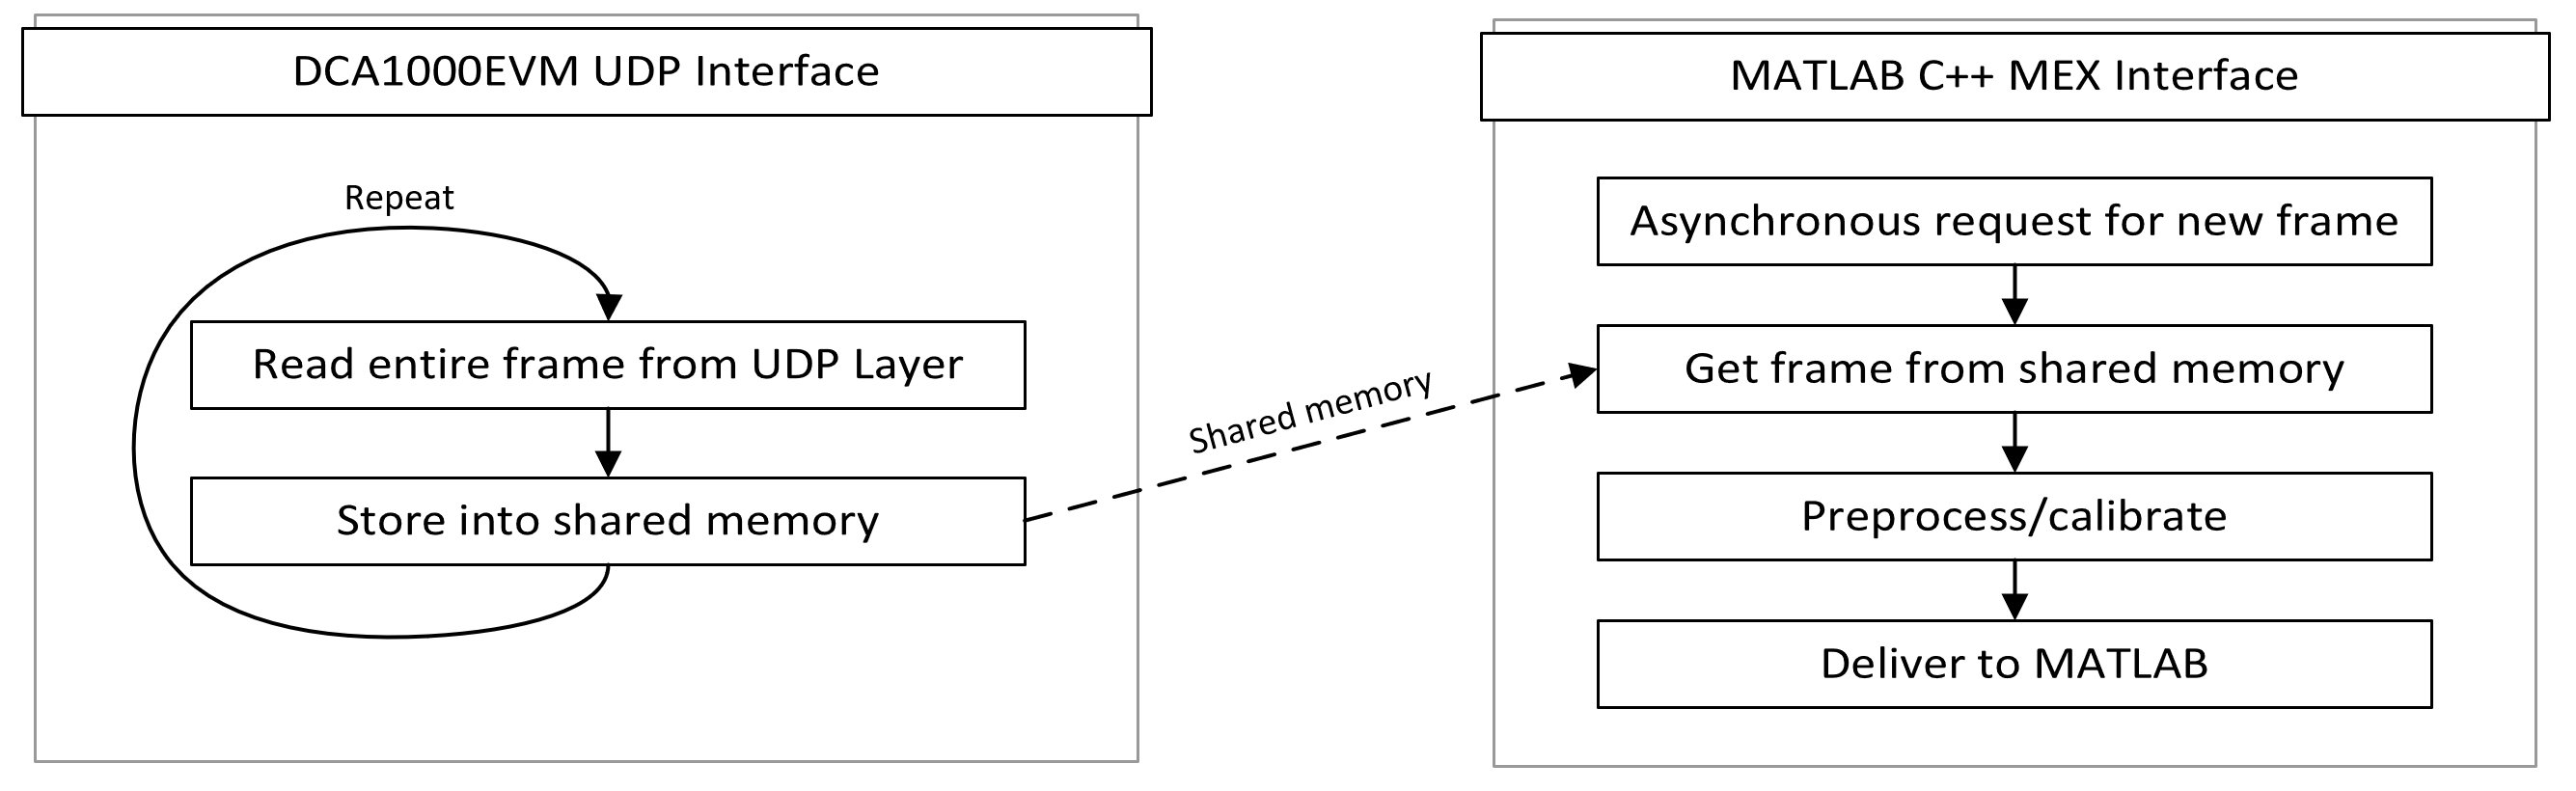
\includegraphics[width=3.6in]{data_retrieval_logic.png}
	\caption{Dual thread logic of custom real-time data retrieval software for direct interface with the DCA1000EVM data capture adapter via UDP layer communication and data delivery to MATLAB.}
	\label{fig:data_retrieval}
\end{figure} 

A custom real-time MATLAB graphical user interface (GUI) is written to serve as the single user interface required for any musician to easily use the Radar Musical Instrument. The MATLAB GUI interfaces with the TI mmWave Studio software \cite{TI:mmWave_Studio} to set up the radar board and data capture adapter, and then initializes the DCA1000EVM UDP interface software to properly read in each packet and organize them into frames based on the user-specified radar parameters. Additionally, by controlling mmWave Studio, the GUI can start and stop capture sequences. While the radar is continuously capturing responses of the target scene, the beat signal is read into the data retrieval software and is delivered to MATLAB. Even though MATLAB does not offer tremendous computational efficiency, it is fast enough to read in frames at a relatively high rate ($50$Hz-$250$Hz). In addition to the beat signal, the MEX function also delivers the frame index to MATLAB our implementation to track when frames are skipped. At this point, the custom MATLAB GUI serves several purposes. First, the GUI is capable of visualizing the range, cross-range, Doppler velocity, and cross-range oscillation in real-time. And finally, the GUI enables precise mapping from the dynamic gestures of the musician to audible notes and a MIDI interface. A custom real-time audio output routine is implemented using the MATLAB Audio Toolbox. Alternatively, the GUI has the option of outputting each feature as to a virtual MIDI device accessible by another program. The custom MATLAB GUI functions either as an end-to-end instrument providing the entire interface, signal processing, and audio output functionality or as a MIDI interface enabling portability and continuity among a multitude of applications and musical venues.

\begin{figure}[h]
	\centering
	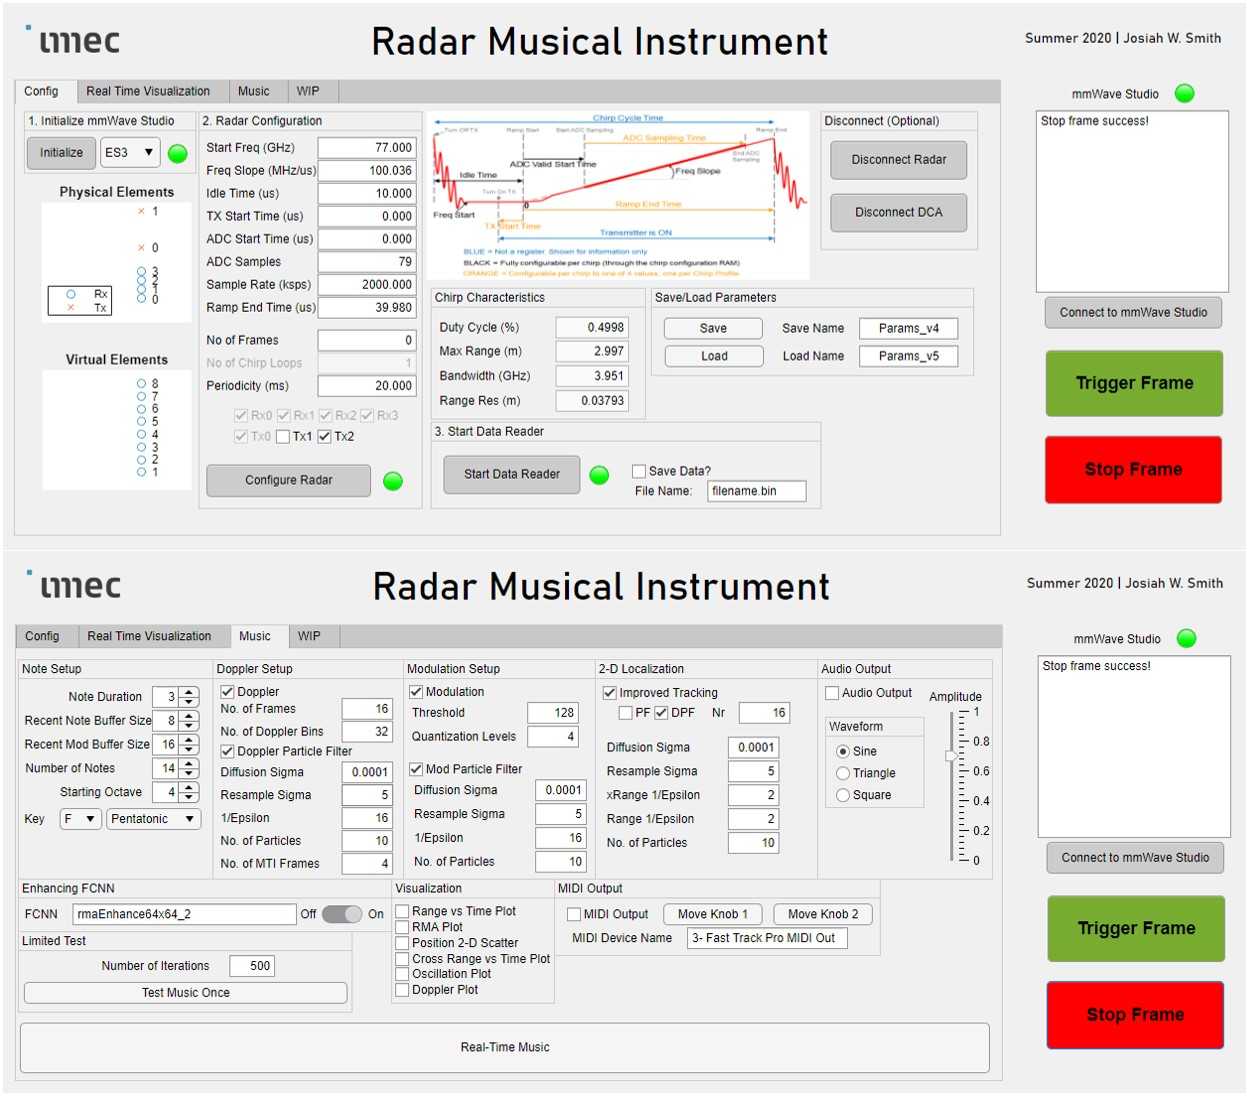
\includegraphics[width=3in]{MATLAB_GUI_2.jpg}
	\caption{Radar Musical Instrument custom MATLAB GUI: device setup and music generation pages.}
	\label{fig:matlab_gui}
\end{figure}

\subsection{Simple Gesture Tracking}
\label{subsec:classical_gesture_tracking}
This section presents the fundamentals of the Radar Musical Instrument. In its most basic form, the Radar Musical Instrument monitors the spatial and temporal signatures of the musician's hand as it is moved throughout the scene converting these features to music. The three parameters controlling the Radar Musical Instrument audio output are range, cross-range oscillation, and Doppler velocity.

For localization, the RMA is used to reconstruct a 2-D image of the hand in the $y$-$z$ plane, as discussed in section \ref{subsubsec:rma}. Once the image is reconstructed and cropped to the user-specified region of interest, a simple peak finding routine locates the peak and estimates the 2-D position on a discrete $y$-$z$ grid. This type of image reconstruction and peak finding suffers from several key factors. First, due to limited bandwidth and number of antennas, the range and cross-range resolution are on the order of centimeters, even without the presence of noise. Additionally, the RMA assumes an ideal beam pattern from a monostatic full-duplex array, but the physical setup consists of antenna elements with varying, non-ideal near-field beam patterns and a multistatic MIMO array. Whereas the multistatic effects can be somewhat compensated for using the phase correction discussed in section \ref{subsec:signal_model}, noticeable image degradation occurs at some positions due to the RMA's monostatic array assumption. These challenges will be further addressed in section \ref{subsec:enhanced_gesture_tracking}.

Despite the non-ideal imaging environment, the 2-D position of the hand can be estimated within several centimeters. Then the range and cross-range position are stored into circular buffers. The real-time position estimate is used to control musical output. To select a note, the musician moves their hand vertically through the region of interest. Instead of selecting from a continuous range of frequencies, "virtual frets" are implemented to quantize the range into subregions corresponding to predefined notes. The note selection and virtual fret parameters are all customizable in the Radar Musical Instrument GUI.

Next, as the cross-range location is stored, its oscillation rate is extracted. Due to possible timing issues in the data retrieval tool discussed previously, a non-uniform fast Fourier transform (NUFFT) is performed is used to extract the oscillation rate. Similarly, a NUFFT is implemented to extract the Doppler velocity as discussed in section \ref{subsubsec:doppler_rma}. 

These temporal features can serve several purposes for musical output. Using the built-in audio output tool, the cross-range oscillation rate is used to control the vibrato specified to each note. If the musician is moving their hand back and forth along the $y$ axis, the Radar Musical Instrument plays the desired note with a vibrato effect at the same rate as the hand. Simply, the frequency of the current note is modulated several Hertz above and below the actual fundamental frequency of the note in a sinusoidal fashion.

Alternatively, the MATLAB GUI is capable of connecting to a virtual instrument via MIDI using range, cross-range oscillation, and Doppler velocity to control the instrument. In this manner, the Radar Musical Instrument acts as a musical interface controlling the software-based instrument similar to a MIDI keyboard. As with the audio output tool, the MIDI output tool discretizes the range into regions corresponding to MIDI notes (whose possible values range from 0 to 127). Now, the cross-range oscillation rate and Doppler velocity are treated as MIDI controller knobs. The musician can program these features to control any tunable parameter within the virtual instrument enabling novel music generation techniques and dynamic control of a MIDI instrument unique to the Radar Musical Instrument. As a result, artists can generate musical sequences in real-time with precise non-contact gesture control that previously was limited to offline programming of a virtual instrument track.

The entire signal processing chain of the Radar Musical Instrument from the input echo signal to the musical features is shown in Fig. \ref{fig:simple_signal_chain}. The echo signal is read into MATLAB where the preprocessing discussed in this section is performed and the user inputs are converted into audio or MIDI output by extracting the spatiotemporal features (range, cross-range oscillation, and Doppler velocity) in real-time. In the next section, these three features are called the new noisy measurements or the new noisy measurement vector $\bm{z}$.

\begin{figure}[h]
	\centering
	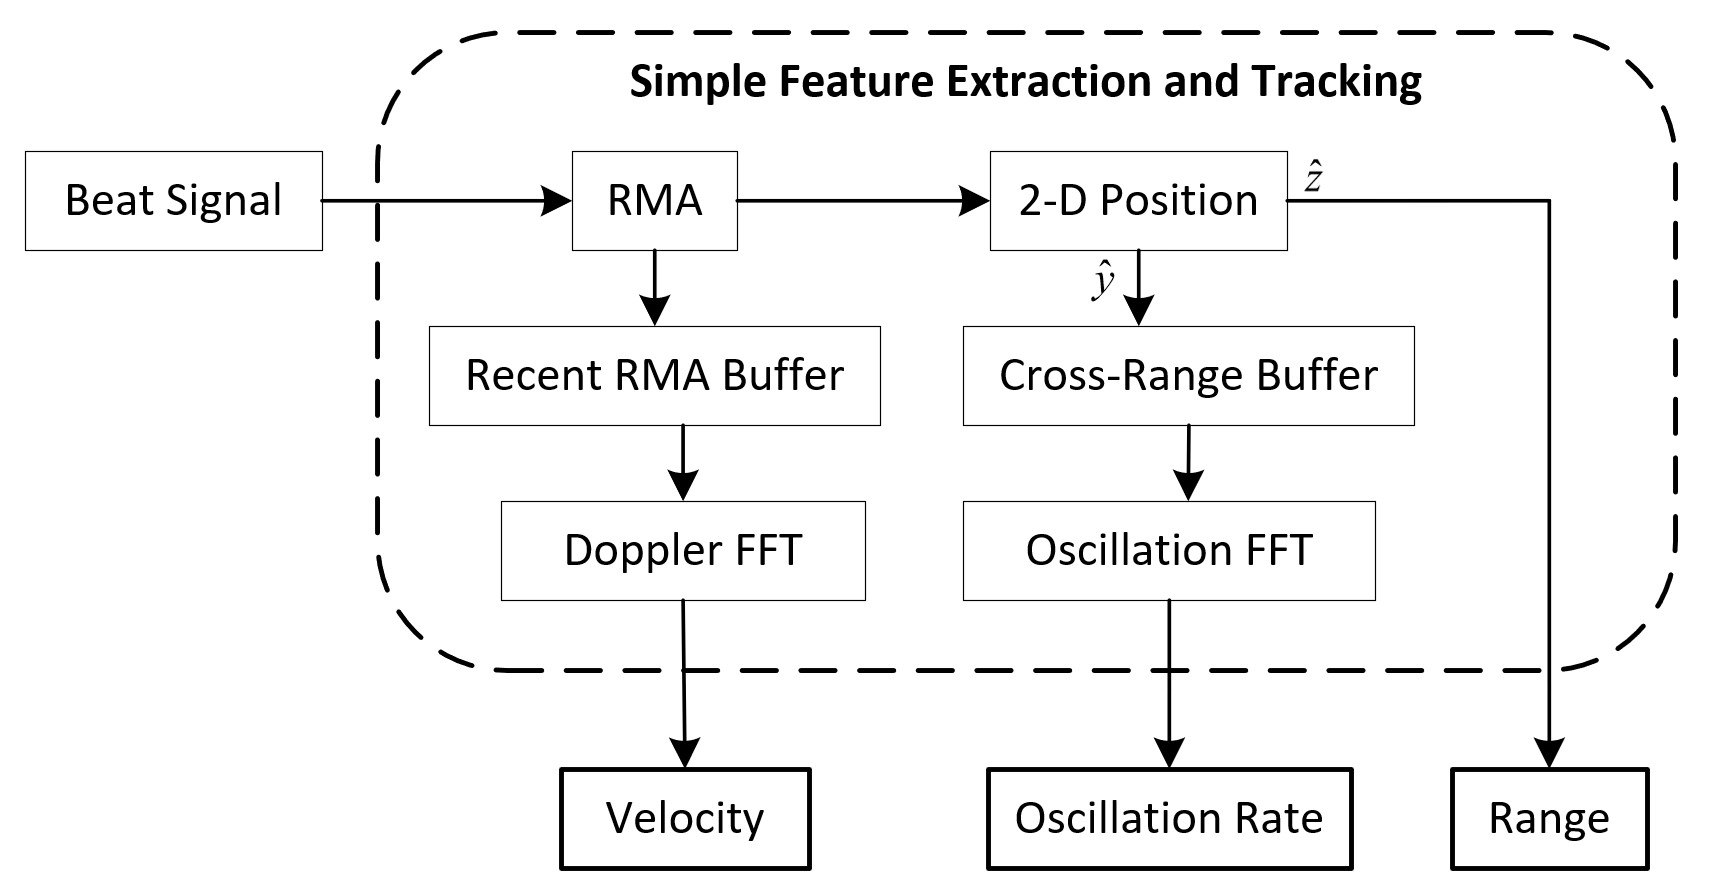
\includegraphics[width=3.3in]{simple_RMI.jpg}
	\caption{Radar Musical Instrument signal processing chain: converting the echo signal input to audio or MIDI output.}
	\label{fig:simple_signal_chain}
\end{figure}

In the simple gesture tracking method, range, cross-range, Doppler velocity, and cross-range oscillation frequency are extracted from the FMCW beat signal using traditional techniques and used to control the musical instrument. Whereas the simple tracking techniques discussed in this section allow tracking of spatial and temporal features, non-idealities due to noise and RMA assumptions degrade RMA image quality and subsequent spatiotemporal tracking performance. We will next demonstrate an improved tracking technique based on a modified particle filter algorithm and deep learning-aided feature extraction method.

\subsection{Enhanced Gesture Tracking}
\label{subsec:enhanced_gesture_tracking}
In this section, we improve the capabilities of the Radar Musical Instrument from the simple tracking techniques to enhanced methods for spatiotemporal tracking and RMA image enhancement to overcome foundational non-idealities in the imaging scenario and inconsistencies in the user input.

\subsubsection{Improved Spatial and Temporal Tracking}
\label{subsubsec:improved_spatial_and_temporal_tracking}
Whereas the simple attempt to track spatial and temporal features of the musician's hand involves estimating the real-time feature as the newest noisy measurement, we improve the Radar Musical Instrument's spatiotemporal tracking robustness by utilizing a modified particle filter algorithm \cite{tracking:condensation_algorithm_radar}. As an example, we begin by employing a particle filter for 2-D spatial localization. A key assumption in our modified model is that the musician's hand is likely to remain in the same location, rather than assuming some constant velocity or known deterministic motion model; we will refer to this assumption the semi-stationary assumption. As a result, our tracking methodology yields highly consistent and smooth localization while finely tracking the hand location throughout the region of interest, but does suffer performance degradation at high hand velocities.

\begin{algorithm}[h]
	\label{algo:particle_filter}
	\SetAlgoLined
	randomize $n$ particle states $\bm{x}_{t-1}$ throughout ROI\;
	initialize $n$ uniform weights $\bm{w}_{t-1}$\;
	\While{true}{
		retieve beat signal $s(y,k)$\;
		extract measurement vector $\bm{z}$\;
		sample particle states $\bm{x}_{t-1}$, with replacement, using weights $\bm{w}_{t-1}$ to obtain $\bm{x}_{t}$\;
		resample particles $\bm{x}_t = \bm{x}_t + \bm{\epsilon} (\bm{z}_t - \bm{s}_{t-1}) + \bm{\psi}$, where $p(\bm{\psi}) \sim N(\bm{0},\Sigma_\psi)$\;
		compute weights $\bm{w}_{t}$ by $p(\bm{z}_t | \bm{x}_t) \sim N(\bm{s}_{t-1},\bm{\Sigma}_w)$\;
		normalize weights $\sum_{n}\bm{w}^{(n)}_t=1$\;
		estimate $\bm{s}_t = \sum_{n}\bm{w}_t^{(n)}\bm{x}_t^{(n)}$\;
	}
	\caption{Modified Particle Filter Algorithm}
\end{algorithm}

Under the semi-stationary assumption, instead of having a deterministic control input, the effective control input is a weighted movement towards the newest measurement. For 2-D localization, the new noisy measurement, stored in the vector $\bm{z}$, is made by performing the RMA and locating the peak. $\bm{z}$ has two elements, the newest estimate of the range, and cross-range. Algorithm \ref{algo:particle_filter} details the modified particle filter implementation, using $\bm{x}$ as the vector containing particle locations in the 2-D plane, $\bm{w}$ as the vector of weights corresponding to each particle, $\bm{z}$ as the measurement vector taken at each time step by extracting the features from the beat signal $s(y,k)$ as described in sections \ref{subsec:classical_gesture_tracking} and \ref{subsec:enhanced_gesture_tracking}, $\bm{s}$ as the estimated state vector, and $N(\bm{\mu},\bm{\Sigma})$ as the multivariate Gaussian distribution with mean vector $\bm{\mu}$ and covariance matrix $\bm{\Sigma}$.

Proper handling of the key steps, 1) resampling of the particle states and 2) computing new weights, is integral to effectively implementing the semi-stationary modification to the particle filter algorithm. 

The particle resampling process involves moving the particles towards the new measurement by a specified weight. $\bm{\epsilon}$ is a diagonal matrix whose elements weight the importance of each new noisy measurement for the corresponding feature. In this way, the new measurements do not dominate the motion tracking but are included in the localization procedure while bypassing the requirement of a motion model. Fig. \ref{fig:particle_filter} demonstrates the resampling process with $\bm{\epsilon} = \frac{1}{2}\bm{I}$, where $\bm{I}$ is the identity matrix. Note that prior computing the new weights, particle diffusion is performed by adding the zero-mean Gaussian noise term $\bm{\psi}$.

\begin{figure}[h]
	\centering
	\includegraphics[width=3.3in]{particle_filter_resample.png}
	\caption{A visual example of the modified particle filter algorithm resampling process. The particle locations are resampled by a shift transformation towards the new measurement according to the diagonal elements of the weight matrix $\bm{\epsilon} = \frac{1}{2}\bm{I}$. }
	\label{fig:particle_filter}
\end{figure}

The new weights are computed from the multivariate Gaussian distribution with $\bm{s}_{t-1}$, the previously estimated states, as the mean vector and a predefined covariance matrix. Therefore, particles closer to the previously estimated state have a higher weight than those farther away. This results in a tendency towards small changes in the state estimations while monitoring for movement from the current position. For many applications requiring precise and consistent localization and motion tracking, our modified particle filter algorithm is an ideal fit as it tends to a steady-state estimation of the states but remains active in monitoring the noisy sensor input.

Just as the 2-D position can be robustly tracked with our modified particle filter algorithm, an identical implementation can be used to estimate and track the velocity of the target and its cross-range oscillation rate as well, both of which are utilized further in the development of the Radar Musical Instrument.

\subsubsection{Doppler-Corroborated Real-Time Weighting}
The resampling and new weight calculation processes result in a similar technique to the Kalman filter with several advantages. It can easily track non-linear dynamics and does not require prior knowledge of the motion model or noise parameters. Now, we extend the constant weighting method to a real-time weighting technique specific for the range domain.
Our approach considers corroboration between the Doppler velocity estimate and the velocity estimated from the range samples as a measure of the new measurement's reliability. Thus, the dependability of the Doppler velocity can improve tracking of the target velocity along the range ($z$) dimension even in the presence of noisy position estimates. First, a Doppler NUFFT is performed across the $N_r$ recent complex RMA images and the Doppler velocity ($\hat{v}_d$) is estimated after video pulse integration by
\begin{equation}
\label{eq:velocity_doppler}
	\hat{v}_d = \arg \max \sqrt{\int |\tilde{d}(z,n_d)|^2 dz},
\end{equation}
where $\tilde{d}(z,n_d)$ is the recent range-Doppler map as discussed previously. Then, the new measurement is used to calculate the sample velocity ($\hat{v}_s$) based on the recent range locations using the least squares estimator as
\begin{gather}
	\hat{v}_s = \frac{N_r \sum_i (\tilde{r}_i t_i) - \sum_i \tilde{r}_i \sum_i t_i}{N_r \sum_i (\tilde{r}_i^2) - \left( \sum_i \tilde{r}_i \right)^2}, \\
	t_i = 0, T_{PRI}, \dots , (i - 1)T_{PRI}, \dots , (N_r - 1)T_{PRI},
\end{gather}
where $\tilde{r}_i$ is the buffer of recent range estimates. Note that the new range measurement is stored at the end of the recent range estimation buffer, $\tilde{r}_{N_r}$, and all the other elements are the previous estimations by the Doppler-corroborated modified particle filter algorithm.

Now, the difference between the Doppler estimated velocity and sample estimated velocity is computed as $\Delta v = |\hat{v}_d - \hat{v}_r|$ and used in the reward function below to update the weight placed on the new noisy measurement in real-time. 

\begin{equation}
\label{eq:velocity_cost_function}
\epsilon_r (\Delta v)=\begin{cases}
	\epsilon_0 \cos \left(\frac{2\pi T_{PRI} \Delta v}{\lambda_0}\right) \quad &\text{if} \, \Delta v \leq \frac{\lambda_0}{4T_{PRI}} \\
	0 \quad &\text{if} \, \Delta v > \frac{\lambda_0}{4T_{PRI}} \\
	\end{cases}
\end{equation}

When the sample velocity is close to Doppler velocity, $\Delta v$ is quite small and the reward function is close to $\epsilon_0$. In this way, the new measurement is corroborated with the more reliable Doppler velocity and weighted accordingly. Outliers and erroneous measurements contradicting the Doppler velocity are given less importance during the particle resampling process. 

Now, the modified particle filter algorithm can be extended to include Doppler corroboration of the new measurement. Simply, the range resampling weight $\epsilon_r$ is computed by (\ref{eq:velocity_cost_function}) and included in the weighting matrix $\bm{\epsilon}$. 

\subsubsection{Improved 2-D Position Estimation by Enhancing FCNN}
\label{subsubsec:improved_2d_position_esitmation_by_FCNN}
Whereas the Doppler-corroborated modified particle filter algorithm improves the tracking consistency and smoothness, non-idealities such as instrumentation delay, ambient/device noise, multistatic effects, and non-spherical beam patterns remain unaddressed. To solve these issues, we present a fully convolutional neural network (FCNN) for image enhancement that improves the 2-D position estimation and subsequent tracking accuracy. Whereas prior CNN techniques are typically based on far-field assumptions and applied in SAR scenarios with large virtual aperture topologies \cite{sar_cnn:enhance1}, our enhancement FCNN method operates on near-field images, improves localization even with a small virtual aperture of eight elements, and is trained using a novel technique allowing the network to learn the environment and device noise, near-field beam pattern, and multistatic effects.

The architecture adopted in this paper for the enhancement FCNN is shown in Fig. \ref{fig:fcnn_architecture}. Four convolution layers of decreasing kernel size are each followed by a nonlinear Rectified Linear Unit (ReLU) layer. Each convolutional layer is zero-padded such that its output is the same size as the input. 

\begin{figure}[h]
	\centering
	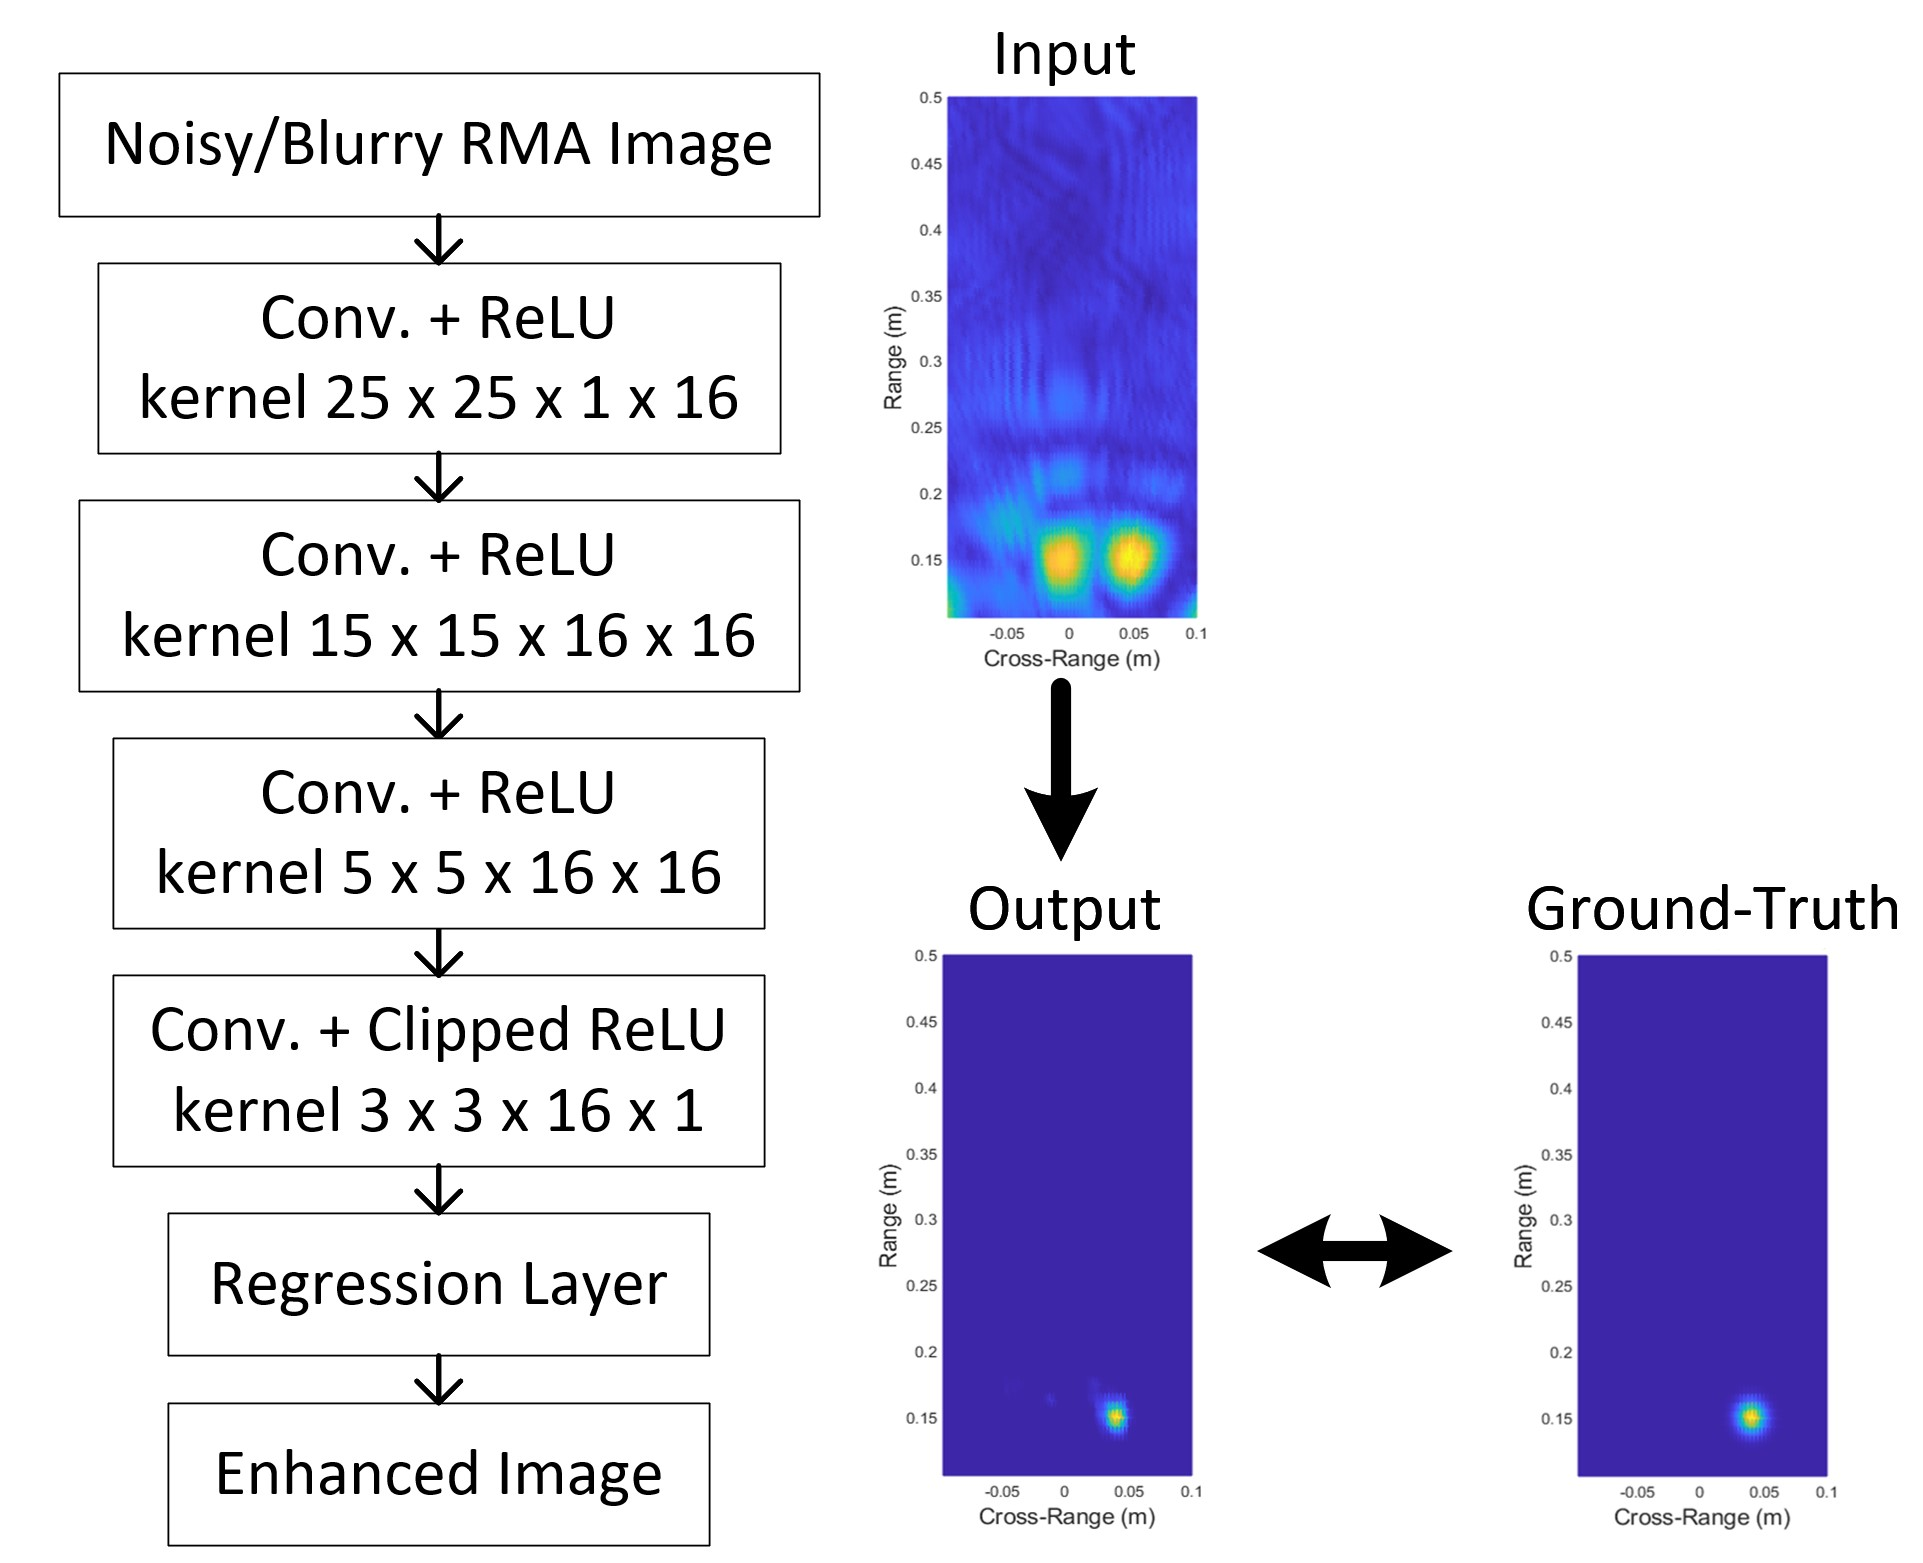
\includegraphics[width=1.4in]{fcnn_architecture.jpg}
	\caption{Architecture of the enhancement FCNN.}
	\label{fig:fcnn_architecture}
\end{figure}

Our enhancement FCNN is trained on both real human hand data and simulated point target data. First, hand data is collected by capturing frames while the user holds their hand at known locations in the ROI. The magnitude of each pixel is taken, $|\hat{p}(y,z)|$, and the real-valued image is the input for training the FCNN allowing the network to fit the non-ideal beam pattern, real multipath and multistatic effects, and actual reflection of a human hand. Next, simulated data is used to supplement the training set. Each simulated sample is generated by simulating a MIMO beat signal with one ideal point target located at a random known location and additive real device noise. The real device noise is captured from the radar with an empty scene. Now, the network learns the device and ambient environment noise as well as the theoretical multistatic effects that remain even after the multistatic-to-monostatic phase correction, thereby improving its generalizability. Our novel training technique results in a robust and generalizable FCNN that improves image signal to noise ratio (SNR) and localization by fitting to the non-ideal imaging constraints. 

The output of the FCNN is generated according to the expected images as modeled by 
\begin{equation}
\label{eq:fcnn_expected_image}
	\mathcal{I}(y,z) = e^{-(y - y_0)^2/\sigma_y^2 -(z - z_0)^2/\sigma_z^2}
\end{equation}
where the width of the expected target located at $(y_0,z_0)$ is dictated by $\sigma_y$ and $\sigma_z$ in the $y$ and $z$ dimensions, respectively, yielding resolutions of $1.18\sigma_y$ and $1.18\sigma_z$ according to the $3$dB beamwidth \cite{sar_cnn:direct1}. The output data is generated requiring knowledge of the exact location of the human hand or point target of each input data sample. During training, the FCNN learns to match each noisy, distorted real-valued RMA image to the expected image learning the various non-idealities inherent to the Radar Musical Instrument scenario. Once trained, the network denoises the RMA images and provides a narrow peak at a more precise location allowing for improved localization and subsequent tracking. Results are presented in section \ref{sec:results}.

Additionally, the enhancement RMA image can be multiplied element-wise by the complex-valued RMA to isolate the complex-valued peak from the hand and mitigate clutter and noise. As a result, the Doppler velocity spectrum SNR is improved, as shown later, since clutter and noise, whose phase adversely affects the Doppler estimation, are greatly reduced. In this way, the enhancement FCNN improves both the spatial and temporal feature estimation in real-time. Pairing the enhancement FCNN with the Doppler-corroborated modified particle filter algorithm, the signal processing chain for the enhanced gesture tracking enabled Radar Musical Instrument is shown in Fig. \ref{fig:enhanced_signal_chain}. 

\begin{figure}[h]
	\centering
	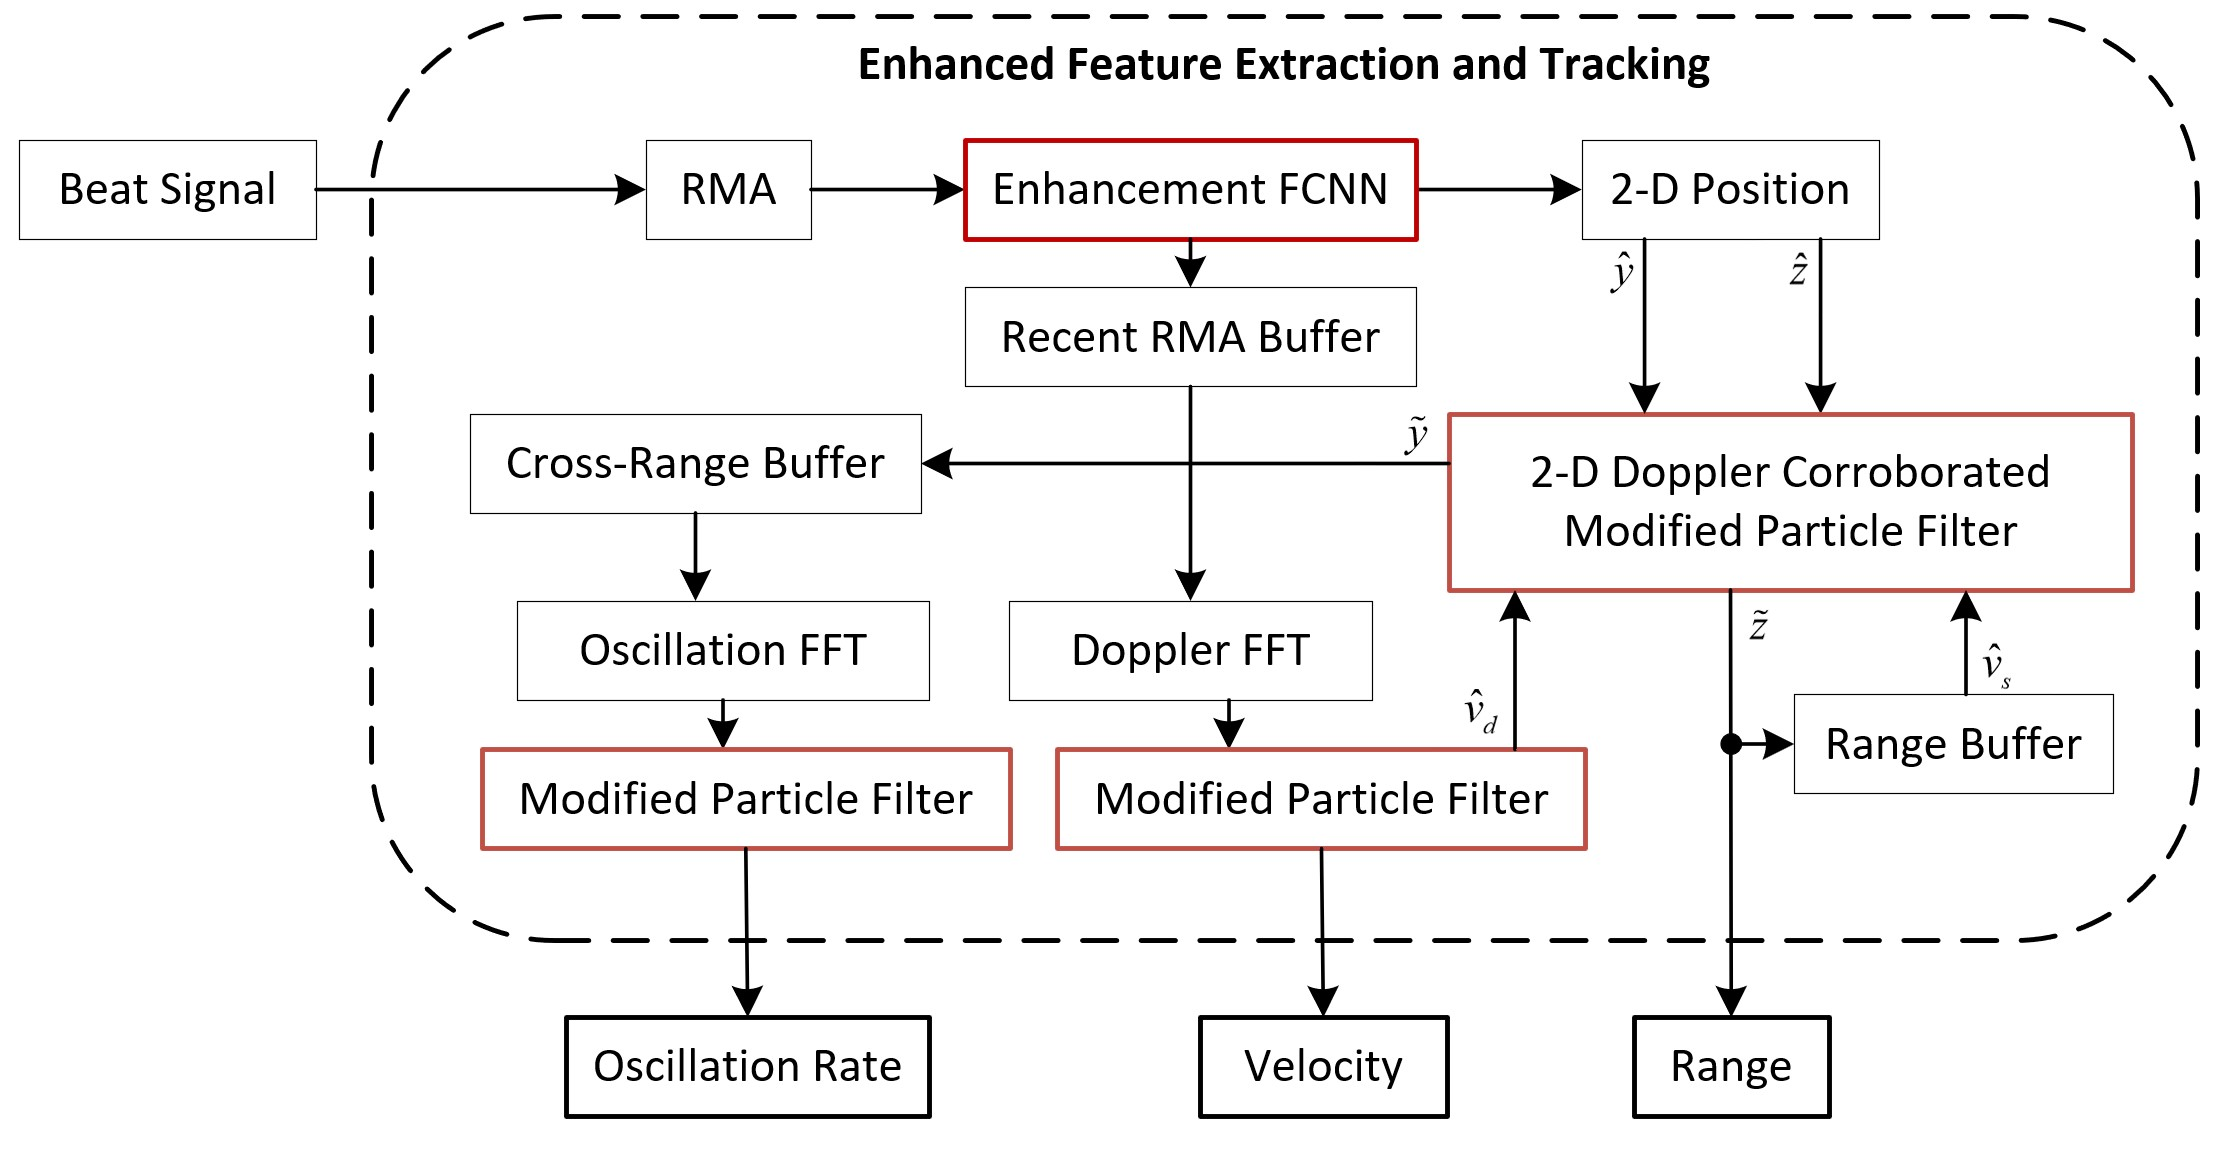
\includegraphics[width=3.3in]{enhanced_RMI.jpg}
	\caption{Radar Musical Instrument signal processing chain from input to musical output now with enhanced gesture tracking by including the Doppler-corroborated modified particle filter algorithm and the enhancement FCNN. Key elements to the enhanced tracking signal processing are highlighted in red.}
	\label{fig:enhanced_signal_chain}
\end{figure}

Utilizing the modified particle filter algorithm and its extension to include Doppler-corroboration improves the robustness of the gesture tracking allowing the Radar Musical Instrument to finely track acute hand gestures even in the presence of noisy user input. Furthermore, the inclusion of the enhancement FCNN enables highly precise position estimation by learning the non-idealities in the device itself and the environment.

\section{Results}
\label{sec:results}

\subsection{Simple Gesture Tracking Results}
\label{subsec:simple_gesture_tracking_results}
As discussed in the previous section, the simple gesture tracking method relies on the traditional techniques presented in section \ref{sec:radar_theory_for_musicians} without any additional tracking algorithm. In real-time, the signal processing chain shown in Fig. \ref{fig:simple_signal_chain} is performed, extracting the spatiotemporal features (range, cross-range oscillation, and Doppler velocity) and converting them to musical output via audio or MIDI signals. At each iteration, the states (spatiotemporal features) are estimated directly from the extracted measurements and are therefore prone to erratic behavior. 

\begin{figure}[h]
	\centering
	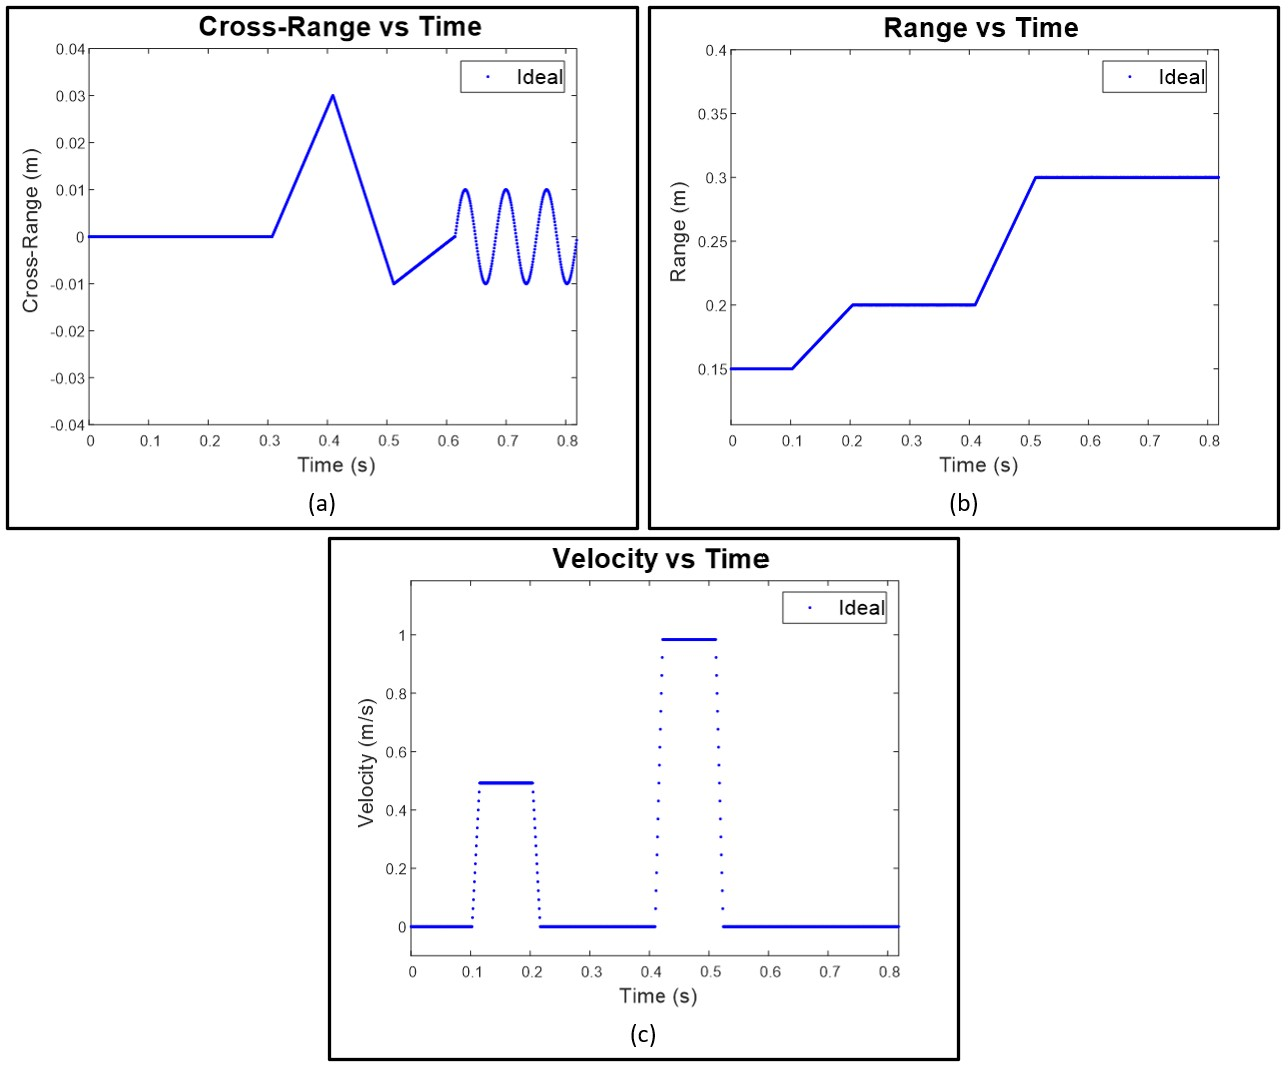
\includegraphics[width=3.3in]{ideal_motion.jpg}
	\caption{Ideal motion profile of the target in the (a) cross-range and (b) range directions as well as the (c) range velocity profile against time.}
	\label{fig:ideal_motion}
\end{figure}

To verify the feature estimation techniques, a virtual prototyping approach is adopted. A point target is simulated in motion with locations and velocity shown in Fig. \ref{fig:ideal_motion} using (\ref{eq:mimo_beat_signal}). Then, real noise collected from the radar with an empty scene is added to each beat signal as
\begin{equation}
	\tilde{s}(y_T,y_R,k) = \frac{p}{R_T R_R}e^{jk(R_T + R_R)} + \alpha \tilde{ \omega}(y_T,y_R,k),
\end{equation}
where $\tilde{ \omega}$ is a complex-valued randomly selected noise sample corrupting the amplitude and phase of the ideal simulated beat signal and $\alpha$ controls the SNR.

The motion profile shown in Fig. \ref{fig:ideal_motion} shows the range ($z$), cross-range ($y$), and velocity of the target. The motion profile includes independent and joint movement in the range and cross-range domains in addition to sinusoidal cross-range oscillation. For our simulations, $4096$ time samples are generated using $p \in [0.5,1]$ to simulate the variance in the hand's empirical radar cross-section (RCS), as observed from prior hand data, and $\alpha \in [1,3]$ to vary the SNR from sample to sample. Values for $p$ and $\alpha$ are selected randomly, within the specified intervals, for each time sample and provide a level of stochastic realism to the simulated data.

\begin{figure}[h]
	\centering
	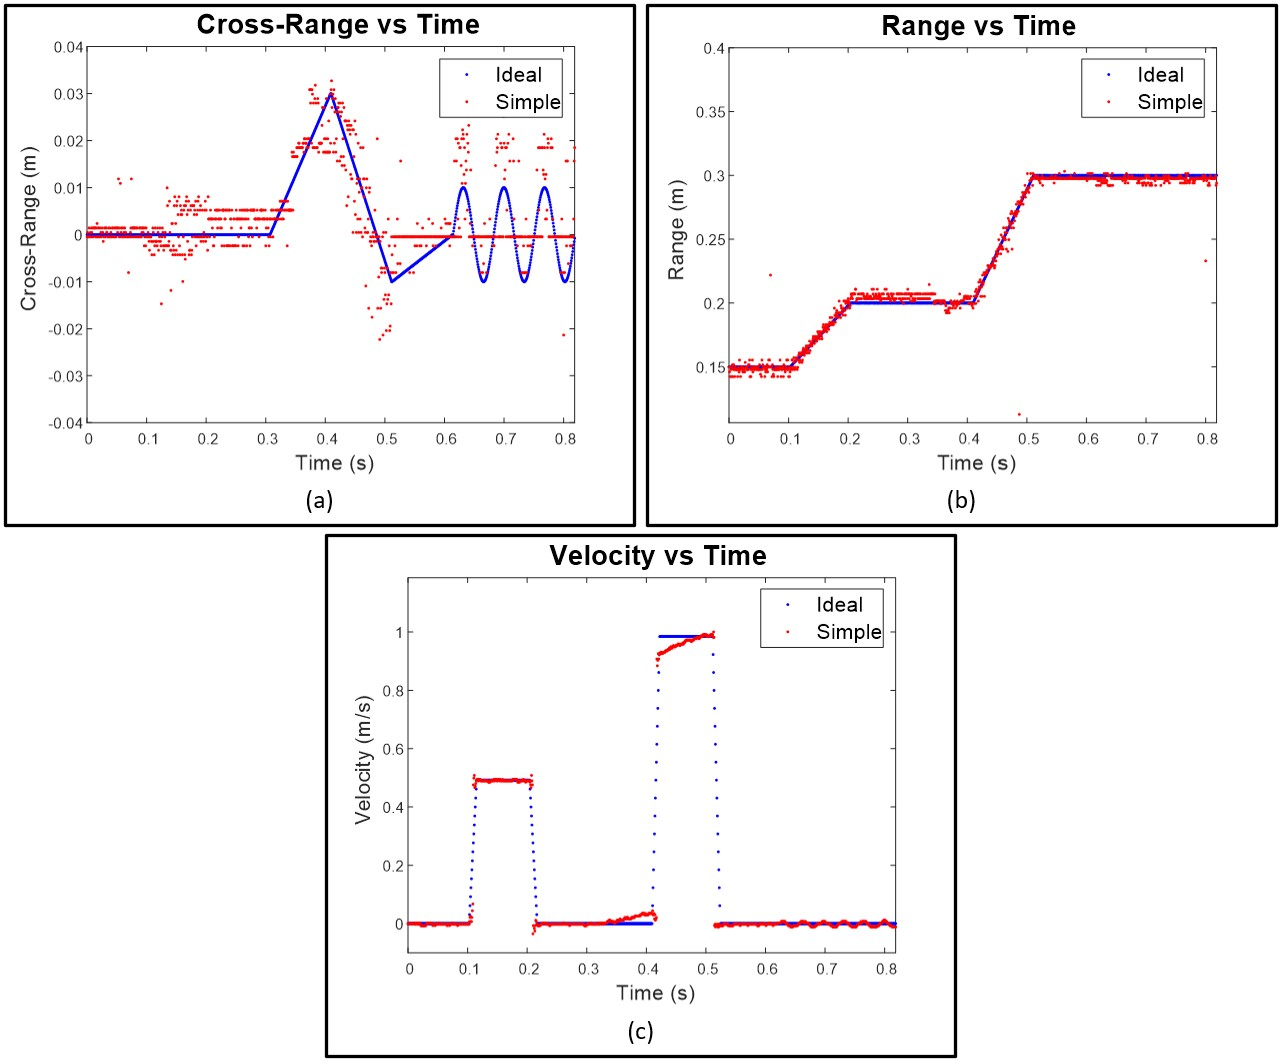
\includegraphics[width=3.3in]{simple_motion.jpg}
	\caption{Motion profile using simple features extraction techniques on each frame for every time step (red) compared with the ideal motion and velocity profiles (blue). The (a) cross-range and (b) range are measured directly from the peak of the RMA image of each frame and the (c) velocity is measured using the Doppler FFT of the raw RMA images using (\ref{eq:doppler_fft}) and (\ref{eq:velocity_doppler}).}
	\label{fig:simple_motion}
\end{figure}

Fig. \ref{fig:simple_motion} shows the features extracted from the simulated noisy beat signals using the simple method. The real radar noise and varying reflectivity result in outliers and errors in the estimated location and velocity of the target. The measurements taken directly from the RMA image generally follow the motion profile and velocity profile of the target, however suffering from an inherently noisy and inconsistent environment. In the following sections, the performance of the simple gesture tracking approach is quantitatively compared to the enhanced tracking method and design considerations are discussed.\footnote{Supplemental material for the reader can be downloaded at http://ieeexplore.org/}

\subsection{Enhanced Gesture Tracking Results}
\label{subsec:enhanced_gesture_tracking_results}
Assuming the same motion profile in Fig. \ref{fig:ideal_motion}, the modified particle filter algorithm is employed in an attempt to more robustly track the 2-D position and Doppler velocity of the target across time, improving the musician's control over the Radar Musical Instrument. 

\begin{figure}[h]
	\centering
	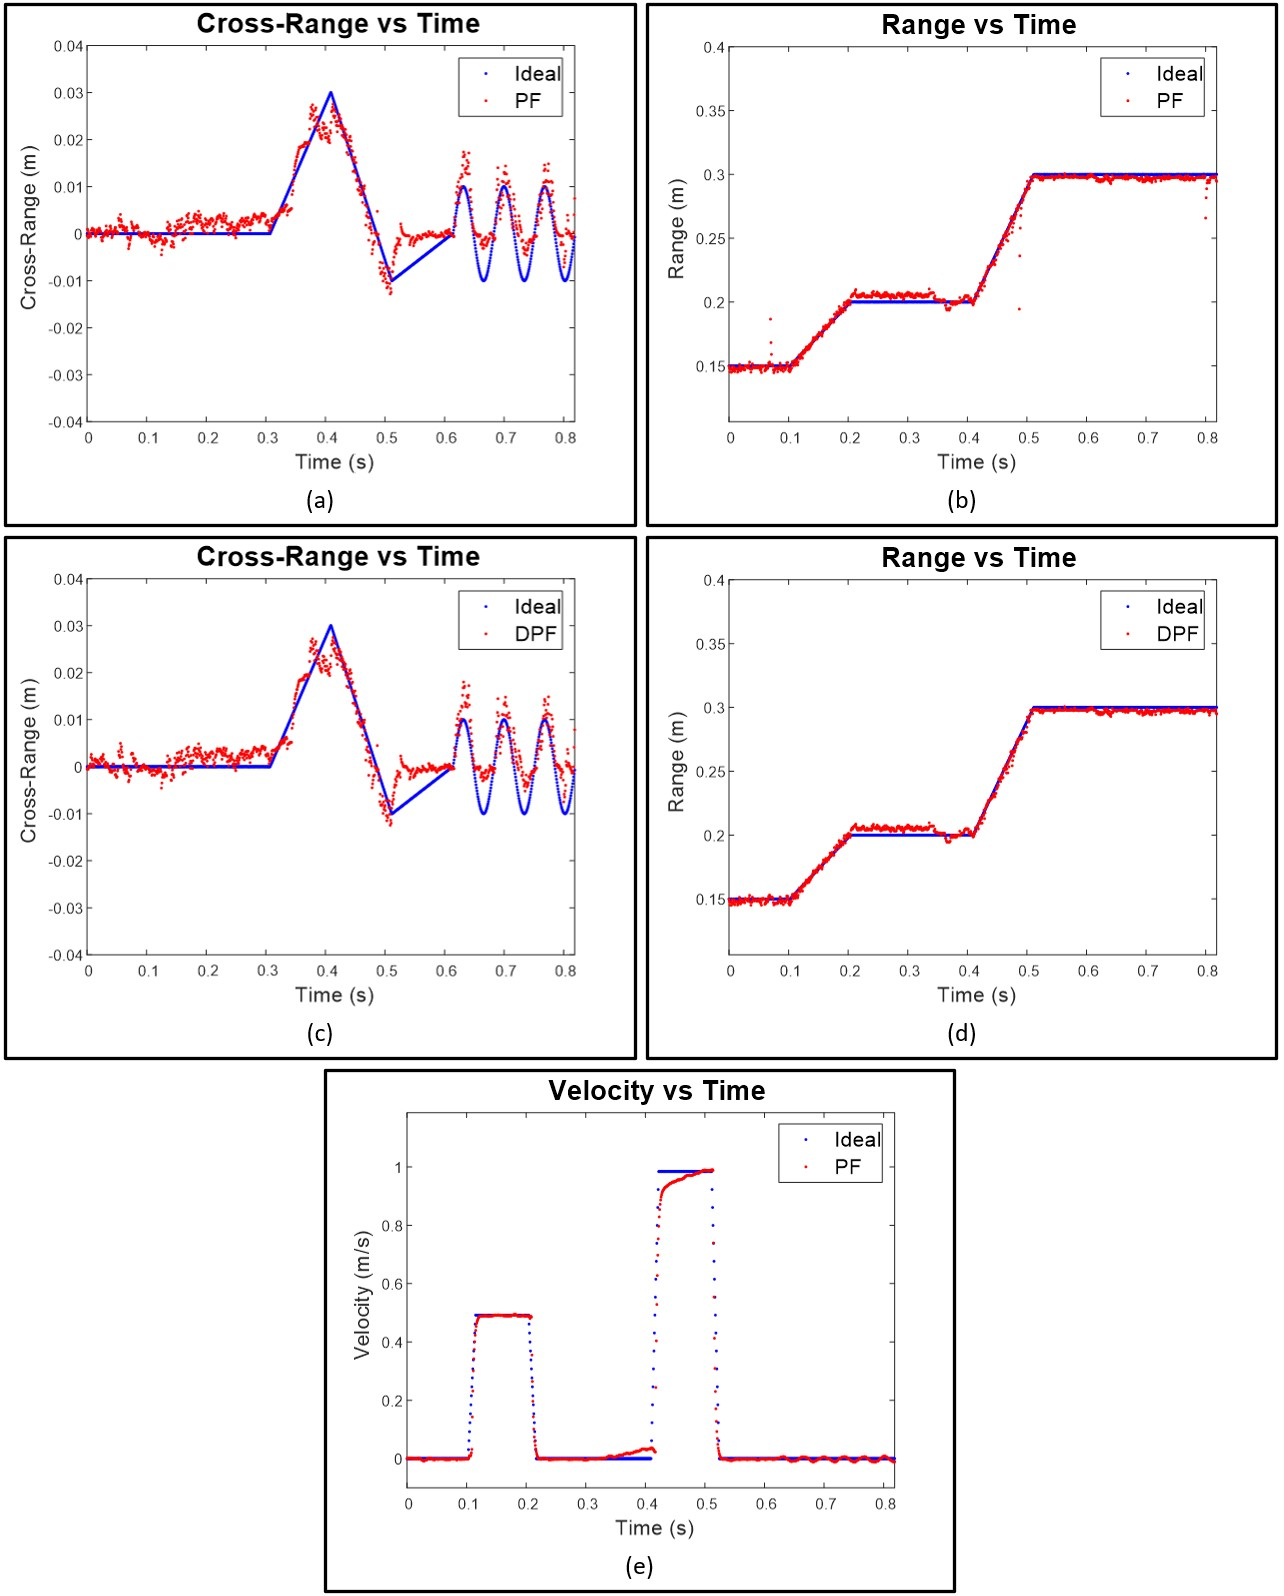
\includegraphics[width=3.3in]{pf_motion.jpg}
	\caption{The modified particle filter (PF) and Doppler-corroborated modified particle filter (DPF) algorithms employed for robust spatiotemporal tracking of the simulated gestures through time: improved tracking of the (a) cross-range and (b) range versus time using the PF, (c) cross-range and (d) range versus time using the DPF with $N_r =$ 16, and (e) Doppler velocity versus time using a PF approach.}
	\label{fig:pf_motion}
\end{figure}

First, the particle filter algorithm (PF) is implemented using the data in Fig. \ref{fig:simple_motion} as elements of the noisy measurement vector $\bm{z}$. The PF reduces the effect of the noise on the position estimation and improves the spatiotemporal tracking performance as shown in Fig. \ref{fig:pf_motion}.

Next, the Doppler-corroborated modified particle filter (DPF) is applied to the same set of data additionally improving the state estimation of the range. Notice the outliers in Fig. \ref{fig:pf_motion}b are mitigated by the DPF in Fig. \ref{fig:pf_motion}d. This is because the outlying samples result in a sample velocity contradicted by the Doppler velocity and weighted as unimportant. The DPF algorithm improves the playability of the Radar Musical Instrument and the user experience by providing a robust, consistent tracking algorithm to smoothly estimate the 2-D position and spatiotemporal signatures of the musician's gestures. However, key issues discussed previously result in degraded RMA images and subsequent noisy measurements reducing tracking performance.

An image-enhancing fully convolutional neural network is implemented to accommodate non-idealities in the device and environment. The enhancement FCNN is trained using both real data from a human hand and simulated data corrupted by additive real radar noise. The FCNN is trained using $65536$ simulated and $23040$ real human hand RMA images as the input and output images with $\sigma_y = \sigma_z = 0.001$m resulting in cross-range and range resolutions of $1.18$mm. Each simulated sample is generated at a random location in the ROI $z \in [0.1,0.5], y \in [-0.1,0.1]$, and the real hand data consists of $512$ samples collected at each of the $45$ locations throughout the ROI as shown in Fig. \ref{fig:fcnn_training_locations}. The simulated samples cover the entire ROI allowing the network to generalize well to location while learning the non-idealities of the imaging scheme.

\begin{figure}[h]
	\centering
	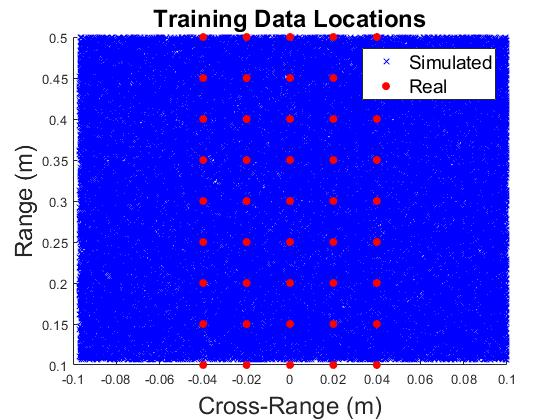
\includegraphics[width=2.8in]{trainingLocations.jpg}
	\caption{Locations of the training data used to train the enhancement FCNN. Real data (red) are collected by keeping the hand static at known locations. Simulated data (blue) are generated by choosing locations randomly from the continuous ROI. Simulated data cover nearly the entire ROI allowing the enhancement FCNN to learn locations throughout the ROI.}
	\label{fig:fcnn_training_locations}
\end{figure}

Training the network for 100 epochs takes 5 hours on a machine with an AMD 3900X processor with 64GB of RAM and a single NVIDIA GTX1080TI graphics card. Other network architectures and training durations are investigated, but this combination yields high performance while offering real-time efficiency.

\begin{figure}[h]
	\centering
	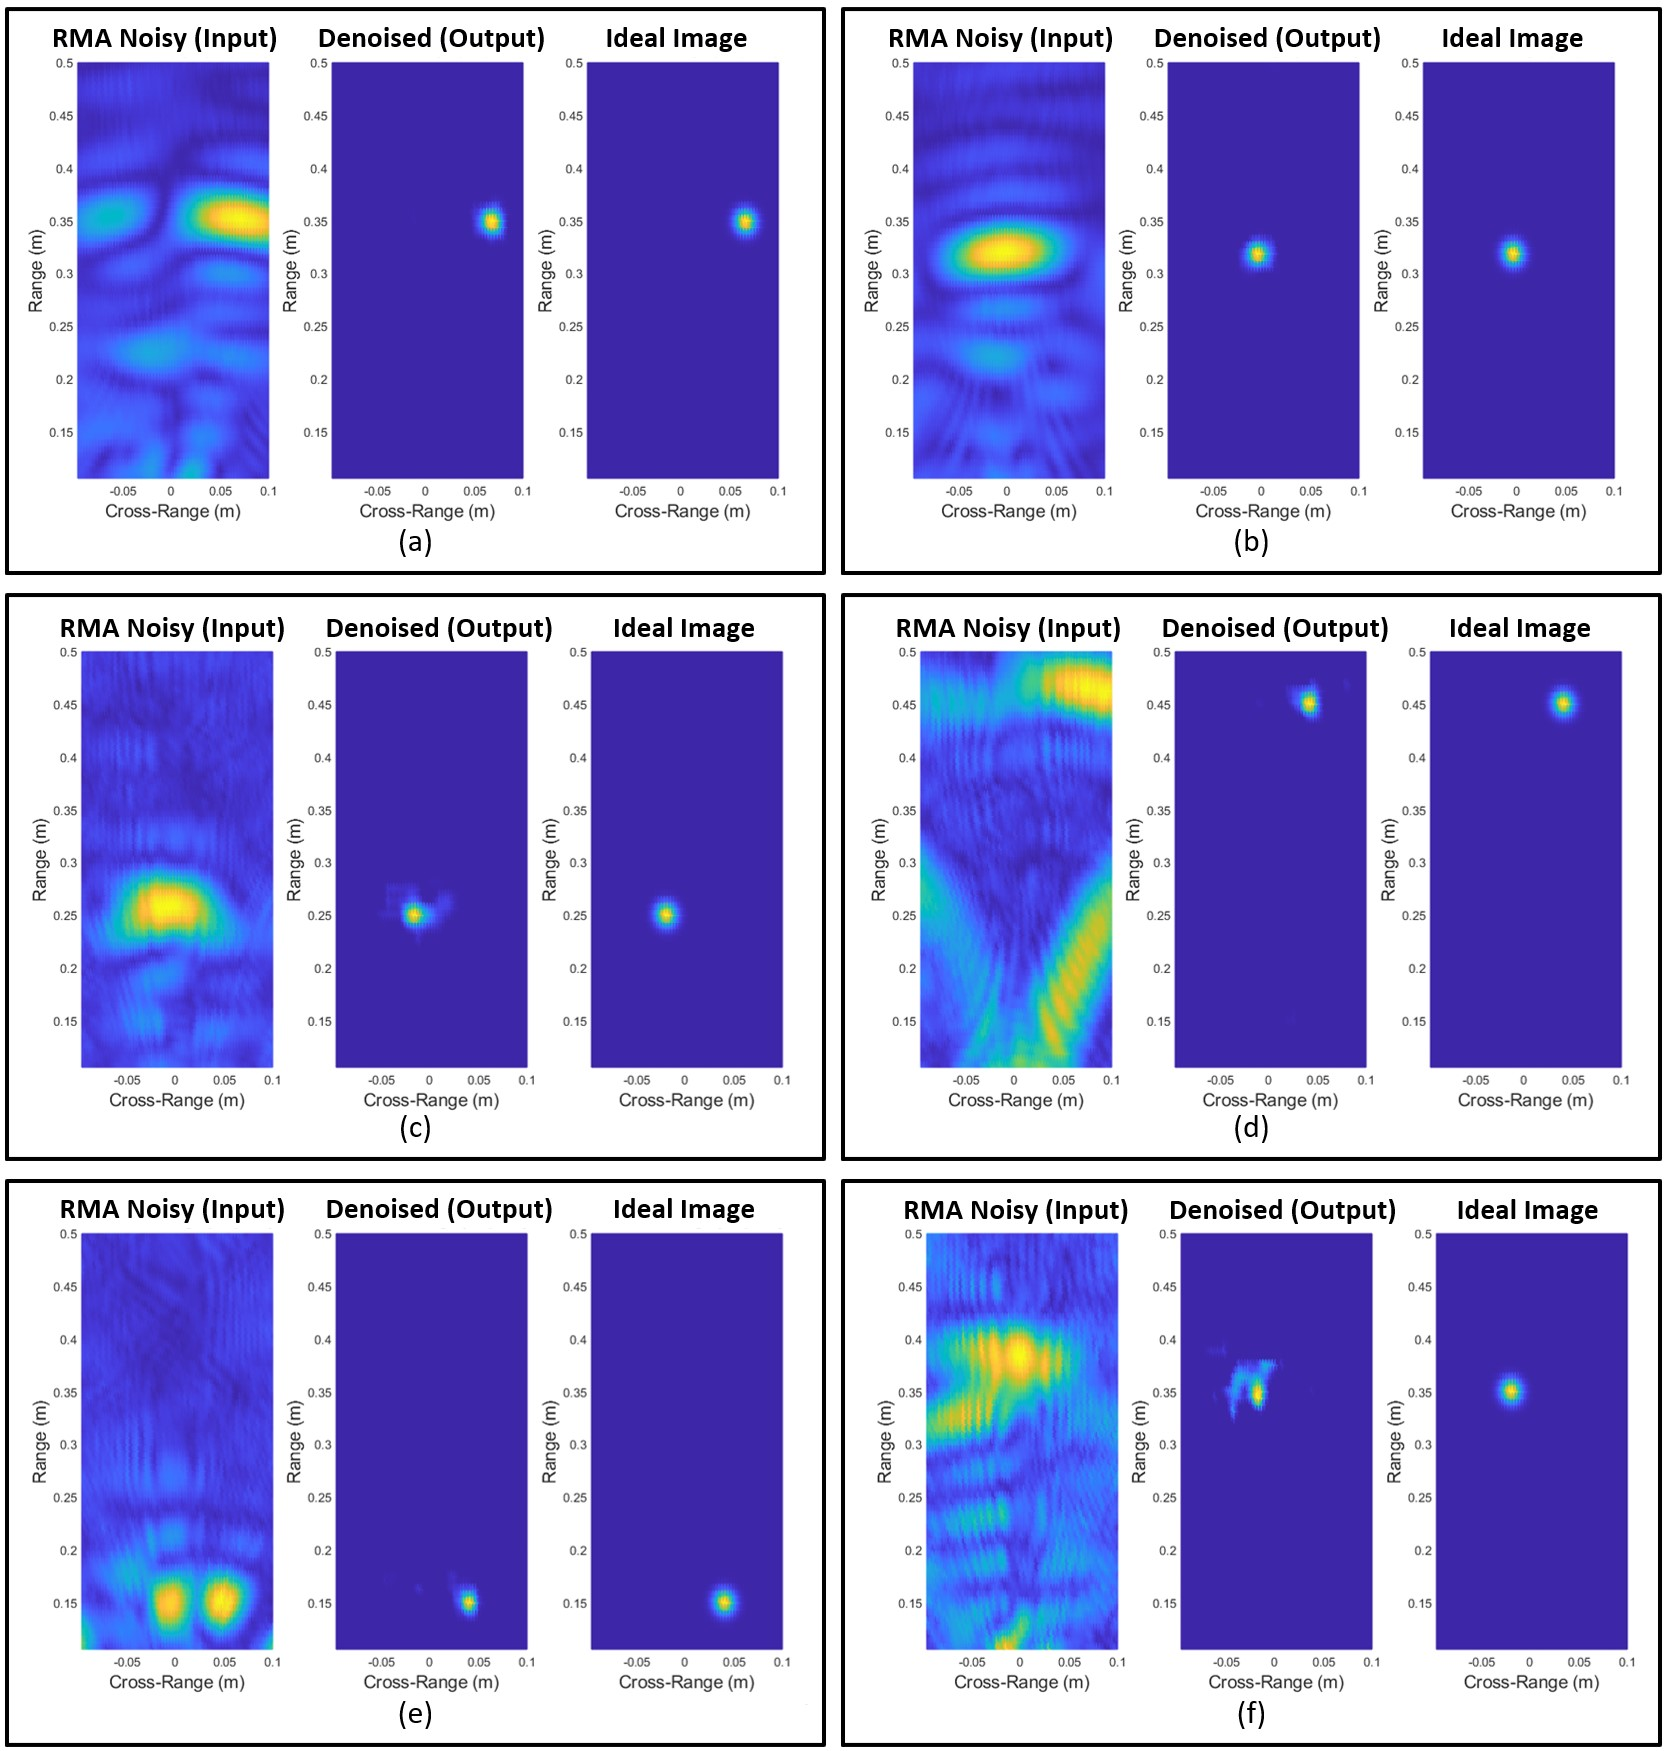
\includegraphics[width=3.3in]{fcnn_results.jpg}
	\caption{Enhancement FCNN applied to simulated (a,b) and real hand (c-f) RMA images for image enhancement and improved localization.}
	\label{fig:fcnn_enhancement_demo}
\end{figure}

Now, a dataset similar to the training set is collected and simulated for validation. Fig. \ref{fig:fcnn_enhancement_demo} shows the images enhanced by the enhancement FCNN demonstrating the robustness of the network. Figs. \ref{fig:fcnn_enhancement_demo}a and \ref{fig:fcnn_enhancement_demo}b show simulated point targets denoised by the FCNN resulting in improved resolution and more precise localization in the denoised image. Fig. \ref{fig:fcnn_enhancement_demo}c is an RMA image reconstructed from a real hand capture close to the middle of the cross-range domain. The 2-D position of the hand is accurately located compared with the ideal image. Similarly, Figs. \ref{fig:fcnn_enhancement_demo}d-\ref{fig:fcnn_enhancement_demo}f demonstrate the network's capability to enhance images degraded by small hand RCS in comparison to noise, the non-ideal beam pattern of each element resulting in ghosting, ambient and device noise, or other non-idealities.

\begin{table} [h]
	\caption{Simple vs Enhanced Localization RMSE}
	\centering
	\begin{tabular}{c || c c}
		\hline
		& $y$ (m) & $z$ (m) \\
		\hline\hline
		Simple & 0.0154 & 0.023 \\ 
		\hline
		Enhanced & 0.0085 & 0.0083 \\ 
		\hline
	\end{tabular}
\label{table:fcnn_position_rmse}
\end{table}

To quantitatively compare the localization improvement of the enhancement FCNN compared to the simple method, the RMSE in the range and cross-range position is computed on the validation dataset using the two techniques and shown in Table \ref{table:fcnn_position_rmse}. The enhancement FCNN not only improves the resolution of the RMA images but results in more accurate and precise localization for both simulated and real data. Applying the enhancement FCNN can further improve the tracking of the spatiotemporal features.

\begin{figure}[h]
	\centering
	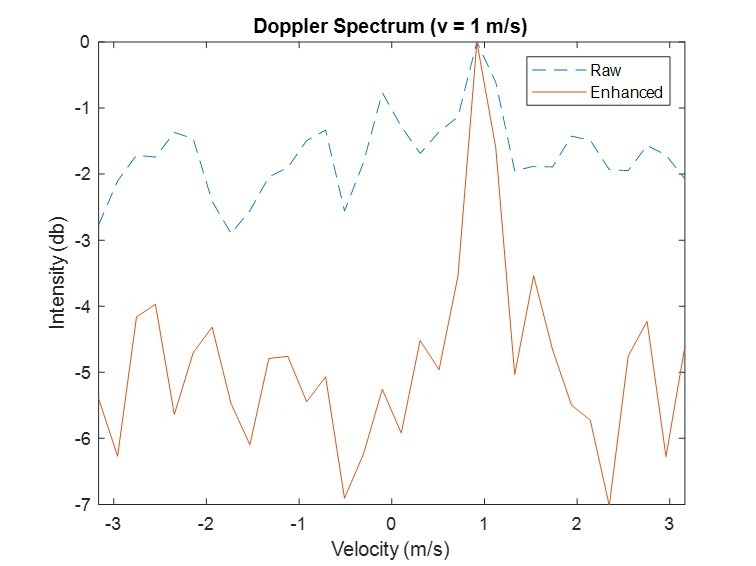
\includegraphics[width=3in]{dopplerSNR.jpg}
	\caption{Comparison of the Doppler velocity spectrum when the Doppler FFT and video pulse integration steps are performed on the raw RMA images compared to the enhanced RMA images. The simulated data contains 128 frames and uses $\alpha = $ 3 for every capture to simulate a low SNR scenario.}
	\label{fig:doppler_snr}
\end{figure}

First, the network improves the Doppler velocity spectrum SNR. Following the signal processing chain in Fig. \ref{fig:enhanced_signal_chain}, the real-valued enhanced RMA image is multiplied element-wise with the complex-valued raw RMA image to preserve the target velocity phase term while mitigating noise and clutter. As shown in Fig. \ref{fig:doppler_snr}, the Doppler spectrum SNR is improved when the Doppler processing is performed on the enhanced RMA images as compared with the raw RMA images, reducing the likelihood of erroneously estimating the velocity. As a result, the enhancement network improves the reliability of the Doppler velocity estimation aiding spatial tracking.

Additionally, the enhancement FCNN improves the tracking accuracy of the Doppler-modified particle filter tracking by improving localization accuracy and dependability of the Doppler velocity. The FCNN enhanced Doppler-corroborated modified particle filter algorithm is abbreviated by FCNN-DPF. Fig. \ref{fig:fcnn_dpf_motion} demonstrates the tracking using the enhancement FCNN paired with the DPF on the same data as the previous tracking examples. Now, the range and cross-range tracking of the target is nearly identical to the ideal motion profile and an improvement in the velocity estimation.

\begin{figure}[h]
	\centering
	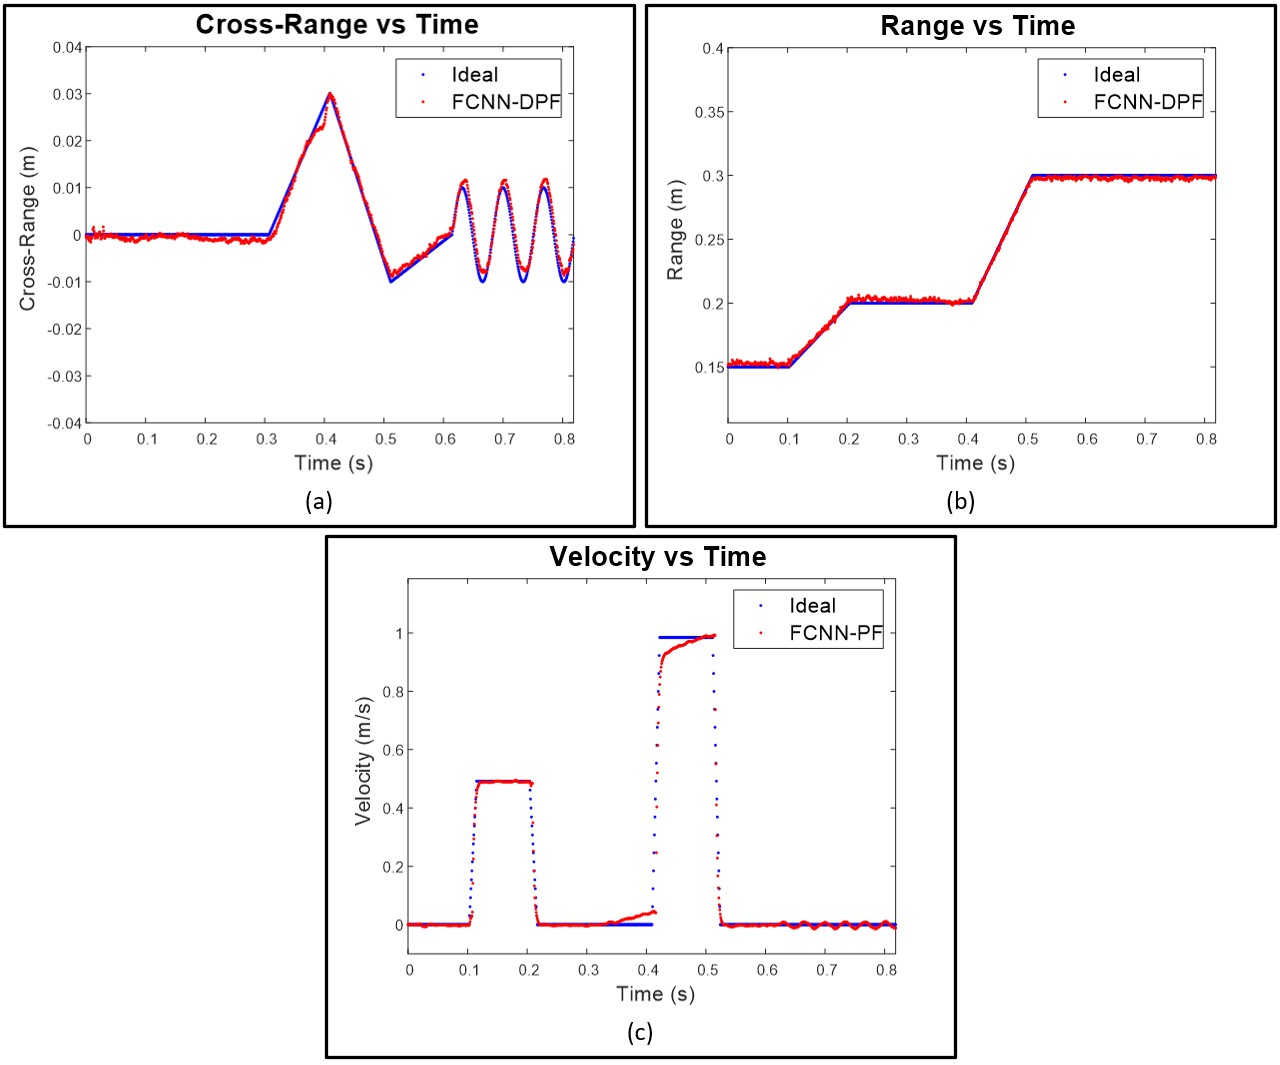
\includegraphics[width=3.3in]{fcnn_dpf_motion.jpg}
	\caption{The FCNN enhanced Doppler-corroborated modified particle filter algorithm.}
	\label{fig:fcnn_dpf_motion}
\end{figure}

To quantitatively compare the tracking performance among the various methods described, $4096$ unique motion profiles are generated and corresponding tracking RMSE is computed for the cross-range, range, and velocity. Displayed in Table \ref{table:tracking_rmse2}, the RMSE for the cross-range ($y$), range ($z$), and velocity ($v$) improve with the novel algorithms proposed in this paper. 

As expected, the simple method yields the greatest error for all three features. Comparing PF and DPF, the cross-range and velocity RMSE are identical between the two techniques but the range RMSE is improved due to the real-time range importance weighting. The FCNN alone outperforms the simple method but can be improved by including the PF and DPF after image enhancement. Finally, the FCNN-PF and FCNN-DPF yield identical results for the cross-range and velocity RMSE, as expected, but significant improvement can be noted in the range RMSE. The results in Table \ref{table:tracking_rmse2} demonstrate the considerably superior tracking performance of the enhancement tracking methods, namely the FCNN-DPF, compared with the simple tracking techniques.

\begin{table} [h]
	\caption{Average RMSE for Tracking Methods}
	\centering
	\begin{tabular}{c || c c c}
		\hline
		& Cross-Range $y$ (mm) & Range $z$ (mm) & Velocity $v$ (m/s) \\
		\hline\hline
		Simple & 7.8627 & 22.0393 & 0.0724 \\
		\hline
		PF & 5.2667 & 13.6412 & 0.0529 \\
		\hline
		DPF & 5.2667 & 6.8543 & 0.0529 \\
		\hline
		FCNN & 7.7365 & 12.2636 & 0.0584 \\
		\hline
		FCNN-PF & 3.6974 & 7.4431 & 0.0445 \\
		\hline
		FCNN-DPF & 3.6972 & 3.0742 & 0.0445 \\
		\hline
	\end{tabular}
\label{table:tracking_rmse2}
\end{table}

Compared to prior results in the literature, our enhanced gesture tracking methods yield impressive results. Past work using WiFi devices, \cite{mmWave_tracking:WiDeo} achieves at best average range tracking error of $2$cm. Again using the $4096$ simulated motion profiles with added noise, our enhanced gesture tracking technique yields mean range tracking error of $1.89$mm. In \cite{mmWave_tracking:ThuMouse}, a 4GHz bandwidth mmWave sensor is used in conjunction with two optical cameras to achieve a 2-D position RMSE of $1.16$mm, at distances closer than $10$cm. Comparatively, even though our enhanced gesture tracking algorithm yields a 2-D position RMSE of $3.4$mm, it is a unique tracking solution using only radar devices and no optical cameras. Moreover, our method offers a mean range resolution of $1.96$mm, a significant improvement over the $4$GHz bandwidth range resolution of $3.75$cm. At the time of this paper, we are not aware of any other prior work on hand tracking using mmWave devices. To our knowledge, the system proposed in this paper offers unprecedented hand gesture tracking performance using a single mmWave sensor.

The enhanced gesture tracking techniques discussed in this section extend the Radar Musical Instrument from a set of simple spatiotemporal feature extraction methods to an accurate, robust gesture tracking system demonstrating the viability of mmWave technology for precise human-computer interaction.

\section{Discussion and Future Work}
\label{sec:discussion}
The enhanced gesture tracking method outperforms the simple method in localization accuracy, Doppler SNR, and tracking accuracy; however, there are some necessary trade-offs for this performance gain. First, the effectiveness of the enhancement FCNN is limited by its training set. Specifically, the network is trained on images from a specific region of interest. Due to the limited aperture size, the farther the target is from the radar, the wider the target appears to be. Since the enhancement FCNN is only trained on images within the expected region, extending the ROI outside of the trained region results in performance degradation. In contrast, the simple methods are highly flexible but cannot compete with the performance of the enhancement techniques.

Whereas the extension of the modified particle filter algorithm to include Doppler-corroboration improves the tracking robustness, in some cases, it can degrade performance. Since the DPF relies on accurate and current Doppler velocity estimation, the system must operate at a fast enough rate that common velocities are within the resolvable range. Following Fig. \ref{fig:data_retrieval}, the DCA1000EVM UDP Interface thread can operate on the order of milliseconds, but the limitation comes in the time between calls to the MATLAB C++ MEX Interface. The rate at which the system is acquires the most recent frame is dependent on the speed of the signal processing chain between MEX function calls. If the signal processing chain takes too much time, the maximum resolvable velocity can become too small. As a result, real-time tracking performance is degraded since aliasing will occur in the Doppler spectrum domain if the musician's hand is moved too fast. In our work, we found the simple and enhanced methods required similar computation times limiting the frequency of the data retrieval function call to a maximum of around $250$Hz. At a starting frequency of $77$GHz, this yields a maximum resolvable velocity of $0.24$m/s limiting the effectiveness of the DPF when the magnitude of the hand velocity is above this maximum.

When it comes to computational efficiency, the addition of the FCNN and particle filter algorithm increases the computational cost slightly compared to the simple measurement method. However, with GPU acceleration more widely available on most PCs and many MCUs, our comparison shows the impact to be negligible using the proposed algorithms.

Lastly, the limited FOV and number of antennas on the automotive radar used in this research limit the extent and resolution of the cross-range domain. Using an array with more elements or elements with a higher beamwidth would increase the performance of the system. Additionally, the 2-D position tracking techniques presented in this paper could easily be extended to 3-D if a 2-D array is employed allowing an added degree of control to the musical instrument at the cost of a larger array topology.

Whereas other work has been done in the area of depth-based hand gesture tracking, the breakthrough presented in this paper overcomes some key limitations of prior work. A significant amount of prior work on optical systems track hand location \cite{optical_tracking:kinect,optical_tracking:zaman,mmWave_tracking:ThuMouse}, but rely heavily on a model-based approach and require specific lighting conditions to function properly. mmWave sensors offer high resolution 2-D and 3-D localization and imaging in non-line-of-sight scenarios such as the presence of fog \cite{radar:fog}, through-the-wall imaging \cite{radar:through_the_wall_imaging_and_tracking}, and around the corner imaging \cite{radar:around_the_corner1}. Prior work on mmWave devices for hand gesture tracking investigate alternative tracking algorithms but cannot match the performance of the methods in our work specifically in precise 2-D localization \cite{mmWave_tracking:ThuMouse,mmWave_tracking:WiDeo}. 

As for future work, several promising routes are left to be explored. First, further development of high-throughput radar devices will increase the speed of the real-time data capture process, allowing for increased reliance on the Doppler velocity estimations. Using multiple MIMO radars or a larger MIMO array would enable multiple hand interface and further extend the application space of our robust tracking methods. Additionally, the MATLAB-based system implementation in this paper can be implemented on high-speed DSP controllers to create a portable system. Finally, the novel precise gesture tracking algorithms of Radar Musical Instrument can easily be extended to offer an elegant, efficient solution to a host of acute gesture tracking problems. 

\section{Conclusion}
\label{sec:conclusion}

The Radar Musical Instrument successfully demonstrates the viability of acute human hand gesture tracking for human-computer interaction using mmWave sensors. We validated and implemented our real-time spatiotemporal signal processing algorithms and robust tracking algorithms in the form of a musical interface; however, the Radar Musical Instrument demonstrates the broad effectiveness of mmWave technology for a multitude of near-field acute gesture tracking applications. First, a simple feature extraction and tracking method were introduced, followed by an enhanced approach leveraging the Doppler-corroborated modified particle filter algorithm and enhancement FCNN to achieve highly robust and accurate tracking in the presence of ambient noise and offering compensation for device non-idealities and multipath effects. The methods are compared demonstrating noticeable improvement using the FCNN-DPF. Additionally, our work offers superior tracking estimation and localization accuracy compared to prior methods in the literature for both mmWave and optical implementations. The novel Radar Musical Instrument presented in this paper offers an elegant solution to a myriad of contactless human-computer interaction problems far beyond the scope of musical interfaces.

\section*{Acknowledgment}
This work was supported by the imec USA summer internship program. We would like to extend thanks to Dr. Gonzalo Vaca Castano for his insights in developing the particle filter algorithm and computer vision approach.

\bibliography{Radar_Musical_Instrument_Paper}
\bibliographystyle{IEEEtran}

\end{document}